\documentclass[11pt,twoside=off,
bibliography=totoc,listof=totoc,appendixprefix,paper=a4,headings=small]{scrbook} % 'twoside=on' für Druckversion oder 'twoside=off' für Onlineversion

%
% Packages
% -----------------------------------
\usepackage[
  paper=a4paper,
  left=12.5mm,
  right=25mm,
  top=25mm,
  bottom=50mm,
  bindingoffset=10mm]{geometry}		% Seitenränder und Bindungskorrektur einstellen

\usepackage[utf8]{inputenc}         % Umlaute im Text

\usepackage[hyphens]{url}
\usepackage[
  backend=biber,       
  style=authoryear,    
  natbib=true,        
  maxcitenames=2,
  mincitenames=1,
  sorting=nyt,         
  giveninits=true   
]{biblatex}
\addbibresource{Literatur/refs.bib}  % Make sure this path is correct
\usepackage{pdfpages}
\usepackage{chngcntr}
\counterwithout{figure}{chapter}
\counterwithout{table}{chapter}

\usepackage[T1]{fontenc}
\usepackage{lmodern}				% Schriftfamilie
\setkomafont{disposition}{\bfseries}

\usepackage{graphicx} 				% Grafiken einfügen (pdf,png - aber jpg vermeiden)
\usepackage{subcaption}
\graphicspath{{./Bilder/}}          % Pfad zu den Bildern
\usepackage{enumitem}
\usepackage{tikz}
\usetikzlibrary{shapes, arrows.meta, positioning,calc}

\usepackage[final,nopatch=footnote]{microtype}

\usepackage{url}					% URL's formatieren (z.B. in Literatur) 
\usepackage[colorlinks,linkcolor=black,citecolor=black,urlcolor=blue]{hyperref} 				% für Hyperlinks in PDF-Dokumenten   
  
\usepackage{tabularx} 				% bessere Gestaltung von Tabellen
\usepackage{longtable} 		
\usepackage{multicol}				
\usepackage{multirow}
\usepackage{booktabs}
\usepackage{float}
\usepackage{tabularx}
\usepackage{forest}
		
\usepackage[active]{srcltx}

\usepackage{listings}				% Algorithmen

\usepackage{mdwlist}				% Listen

\usepackage{setspace} 				% Zeileneinstellung
\newtheorem{mydef}{Merksatz}  		% Falls Beispiele, Merksätze m. fortl. Nr. gebr. werden
\newtheorem{bsp}{Beispiel}

\usepackage{lscape}					% zum Rotieren von Seiten

\usepackage{amsmath}				% zum Schreiben von mathematischen Formeln
\usepackage{amssymb}   
\usepackage{amsfonts} 

\usepackage{calc}

\usepackage{footnote}				% Fußnoten
\usepackage{tablefootnote}			% Fußnoten in Tabellen
\usepackage{makecell} 

%\clubpenalty = 10000
%\widowpenalty = 10000 \displaywidowpenalty = 10000

\hyphenation{voll-st\"andigen}		% Worttrennungen global definieren

\setcounter{tocdepth}{2}			% Ebenen, die im Inhaltsverzeichnis angezeigt werden

% Document
% -----------------------------------
\begin{document}

\frontmatter 
    % Titelseite soll keine Kopf oder Fußzeile haben
\thispagestyle{empty}

% Alle Elemente sollen zentriert sein
\begin{center}

\vspace*{-10mm}

{\Large \textbf{Detecting Gender Bias in}}\\ 
\vspace*{2mm}
{\Large \textbf{English-German Translations}}\\ 
\vspace*{2mm}
{\Large \textbf{using Natural Language Processing}}\\

\vspace*{\fill} 

{\LARGE {Bachelor's Thesis}}\\ 

\vspace*{\fill} 

for the attainment of the academic degree Bachelor of Science (B.Sc.)\\ \vspace*{1.5mm} 
in the study program\\\vspace*{1.5mm}
\textbf{Information Systems Management}\\\vspace*{1.5mm}
at the\\\vspace*{1.5mm}
Berlin School of Economics and Law\\

\vspace*{\fill} 

% Name des/der Autors/Autoren
{\Large Submitted by Khanh Linh Pham}\\[15mm]

\vspace*{\fill} 

% Gutachter, Kontaktdaten und Abgabetermin
\begin{flushleft}
\begin{tabbing}
Main Supervisor:\hspace{1.6cm} \= Prof. Dr. Diana Hristova \\
Secondary Supervisor:\> Prof. Dr. Markus Schaal \\[4mm]
Semester:\> Summer Semester 2025\\
Matriculation no.:\> 77211916753\\
Email:\> klpham04@gmail.com\\[8mm]
\textbf{Date of Submission:} \> \textbf{xx.xx.2025}\\
\end{tabbing}
\end{flushleft}

\end{center}

\clearpage{\pagestyle{empty}\cleardoublepage} 			% Titelblatt
    \clearpage{\pagestyle{empty}\cleardoublepage}
    \thispagestyle{empty}


\vspace*{1cm}

\begin{center}
    \textbf{Abstract}
\end{center}

\vspace*{1cm}

\noindent 
Gender bias in English–German Machine Translation often appears in forms such as generic masculine defaulting and occupation stereotyping. These biases can perpetuate unequal representations and feed back into future translation models, reinforcing biased outputs in society. This thesis examines how accurately multilingual BERT (mBERT) can detect such bias. The model was fine-tuned on limited datasets with varying annotation quality, which caused its main limitations. The classifier occasionally (1) misclassifies German gender-fair language forms as biased, (2) fails to detect bias in political and government terms, (3) fails to recognize semantically gendered words as unbiased, (4) is sensitive to punctuation and capitalization, and (5) struggles with sentences that contain both neutral and gendered subjects. Despite these gaps, the model achieved an F1 score of 0.966 and proves effective for core bias cases. It reached 84.4\% accuracy on a small handcrafted evaluation dataset with practical sentences like job postings and edge cases. As an intermediary step, the work offers a trained model, sufficiently effective for practical bias detection, and an application that make biased translations visible while indicating areas for further investigation and improvement.
    \newpage
    
    \clearpage{\pagestyle{empty}\cleardoublepage}
    \thispagestyle{empty}


\vspace*{1cm}

\begin{center}
    \textbf{Sperrvermerk}
\end{center}

\vspace*{1cm}

\noindent 

Die vorgelegte Masterarbeit basiert auf internen, vertraulichen Daten und Informationen des Unternehmens ...... In diese Arbeit dürfen Dritte, mit Ausnahme der Gutachter und befugten Mitgliedern des Prüfungsausschusses ohne ausdrückliche Zustimmung des Unternehmens und des Verfassers keine Einsicht nehmen. Von diesem Verbot ausgenommen sind außerdem jene Personen, die auch ansonsten zur Einsichtnahme in die genannten Daten und Informationen befugt sind. Eine Vervielfältigung und Veröffentlichung der Masterarbeit ohne ausdrückliche Genehmigung – auch auszugsweise – ist nicht erlaubt.

\vspace{2cm}

\noindent
Berlin, den 01. Januar 2099

\vspace{3cm}

\hspace*{7cm}%
\dotfill\\
\hspace*{8.5cm}%
\textit{(Unterschrift des Verfassers)}      % Sperrvermerk
    \newpage
    
    \clearpage{\pagestyle{empty}\cleardoublepage}
    \onehalfspacing                  	% Zeilenabstand ab hier 1.5 zeilig
    \tableofcontents 					% Inhaltsverzeichnis
    \clearpage{\pagestyle{empty}\cleardoublepage} 
    
    \listoffigures 					 	% Abbildungsverzeichnis
    \clearpage{\pagestyle{empty}\cleardoublepage}
    
    \listoftables						% Tabellenverzeichnis
    \clearpage{\pagestyle{empty}\cleardoublepage}

    \chapter*{List of Abbreviations}  
\addcontentsline{toc}{chapter}{List of Abbreviations} 
\begin{description}[align=left,labelwidth=3cm]
  \item[EN-DE] English-to-German
  \item[GFL] Gender-Fair Language
  \item[mBERT] Multilingual BERT
  \item[MT] Machine Translation
  \item[NLP] Natural Language Processing
  \item[NMT] Neural Machine Translation
\end{description}

    \clearpage{\pagestyle{empty}\cleardoublepage}

% -----------------------------------
\mainmatter 							% die einzelnen Kapitel
    \chapter{Introduction}
Machine Translation (MT) is a sub-field of computational linguistic that uses computer software to translate texts between languages \citep{linMachineTranslationAcademic2009}. It is a major area within Natural Language Processing (NLP), a branch of Artificial Intelligence (AI) \citep{smacchiaDoesAIReflect2024}. This technology helps millions of people communicate across languages, whether in every situations or high-stakes domains like healthcare, law and business \citep{kapplAreAllSpanish2025}. Users rely on it to translate everything from casual conversations to medical prescriptions and legal documents. Tools like Google Translate serve over 200 million users daily \citep{pratesAssessingGenderBias2019,shresthaExploringGenderBiases2022}, with new advanced translation models appearing on the market frequently. According to a market analysis by \citet{skyquestMachineTranslationMT2025}, the MT market size was valued at 980 million USD in 2023 and is projected to reach 2.78 billion USD by 2023. 

With this growing availability and accessibility of free MT tools capable of handling complex sentences, their use in translating large volumes of online content is increasing \citep{thompsonShockingAmountWeb2024}. This not only expands their influence on global access to information, but also shapes how readers perceive and interpret that content. Automated and unsupervised translations raise new concerns: not just about quality, but also about bias. One aspect is gender bias. Several studies \citep{smacchiaDoesAIReflect2024,choMeasuringGenderBias2019,stanczakSurveyGenderBias2021,soundararajanInvestigatingGenderBias2024} confirm that MT systems trained on large-scale datasets that incorporate societal biases, can learn and perpetuate gender biases present in the training data. In short, if the training data reflects gender stereotypes, the translation system is likely to repeat them. This includes, but is not limited to, the insertion of gendered pronouns in place of originally gender-neutral terms, and the use of stereotypically gendered occupational titles.

There is a risk of incorrect gender assignment when translating between languages with and without grammatical gender. For example, the gender-neutral English sentences "The surgeon is hard-working" and "The nurse is hard-working" are translated into German as "Der Chirurg ist fleißig" and "Die Krankenschwester ist fleißig" respectively, as seen in \autoref{fig:gt_surgeon_example} and \autoref{fig:deepL_surgeon_example}. These translations introduce occupational gender stereotypes. “Der Chirurg” is the masculine form of “surgeon” in German, adding a male gender where the original English sentence did not specify one. Similarly, “Die Krankenschwester” is the feminine form of “nurse,” again assigning a gender that was not present in the source. These patterns are not just technical flaws. They can reinforce harmful stereotypes in real-world contexts. The following section outlines the broader motivation behind this thesis.


\section{Motivation}

Academia has come to the consensus that MT systems do default to male pronouns when gender in the source sentence is ambiguous. In addition, as shown in the earlier example where "the surgeon" and "the nurse" were translated with stereotypical genders, the reinforcement of occupational stereotypes is an increasing concern. When MT is used for job descriptions, recommendation letters, or resumes and it inserts or reinforces unfairly gendered language \citep{bolukbasiManComputerProgrammer2016}, it may discourage individuals whose gender is misrepresented or stereotyped. In turn, this would reduce their chances of success in recruitment processes. 
This may also bring broader consequences for businesses: Failing to address this issue can lead to the exclusion of qualified candidates, reduce diversity and contradict international standards. Organizations like the United Nations, UNESCO, and the European Union stress the importance of gender equality and inclusive language, making gender equality one of the 17 Sustainable Development Goals for 2030 \citep{sczesnyCanGenderFairLanguage2016,unitednationsAchieveGenderEquality2023}.
Ethical AI guidelines from global institutions also highlight the need for fair outcomes \citep{ullmannGenderBiasMachine2022}, therefore businesses need to meet these standards if they want to stay credible and act responsibly. 

Current research on this topic tends to focus more on the quantitative measurement of gender bias \citep{rescignoGenderBiasMachine2023,barclayInvestigatingMarkersDrivers2024a,smacchiaDoesAIReflect2024}, e.g. counting the occurences of gendered pronouns or grammatical forms in outputs when prompting models with a neutral input. It is then often compared against a standard or desired outcome like real-world demographic distributions \citep{smacchiaDoesAIReflect2024,pratesAssessingGenderBias2019} or human evaluation \citep{lardelliBuildingBridgesDataset2024,savoldiWhatHarmQuantifying2024}. However, current evaluations are not enough for accountability. Few approaches address an active gender bias detection layer. While this gap remains in translation systems, similar issues have been addressed in other domains. For example, as summarized by \citet{shresthaExploringGenderBiases2022}, \citet{schwemmerDiagnosingGenderBias2020} propose a detection framework to uncover gender bias in facial recognition technologies. Their findings show that these systems are more accurate in identifying individuals as women when the images conform to stereotypical feminine features like long hair or makeup. In some cases, systems even associated such images with stereotypically gendered labels like "kitchen" or "cake," despite these elements not being present. 
A detection system specifically for MT would increase linguistic transparency, because without the development of bias-aware tools, problematic translations are likely to scale without oversight. Therefore, addressing gender bias in MT becomes both a social and ethical necessity.

\section{Problem Statement and Research Questions}

The core problem boils down to the significant bias towards the masculine form in English-German MTs, sometimes consituting 93-96\% of translations for isolated words \citep{lardelliBuildingBridgesDataset2024}. These outputs often reflect social stereotypes rather than objective translations, yet current systems offer no mechanism to detect or signal when such bias occurs \citep{rescignoGenderBiasMachine2023}. To address this, this thesis deploys a blackbox approach to explore how fine-tuning a pre-trained multilingual BERT model can help detect gender bias in MT outputs. The model takes an input sentence and its corresponding German translation and predicts whether the translation introduces gender bias. It focuses on identifying two common cases: added gendered pronouns and wrongly gendered nouns.

The translation system used is \href{https://github.com/Helsinki-NLP/Opus-MT?tab=readme-ov-file}{Opus-MT}, an open-source neural MT model. %mention which bert i will use% 
Translations are passed through BERT, trained on a dataset I have constructed by combining and adapting several existing datasets from other researchers. The classifier is lightweight and efficient, aiming for transparent behavior and easy integration into other tools \citep{devlinBERTPretrainingDeep2019}. Its predictions are used to highlight biased parts in a web-based demo. The goal is not to build a perfect detector, but a working proof of concept that shows how bias can be flagged automatically. This supports more critical use of MT systems and encourages further development of bias-aware translation tools.

The main research question is: \textbf{How can a NLP-based binary classification model detect gender bias in English-German translations?}. This involves building a suitable training dataset, selecting features that capture bias patterns, and evaluating how well the model generalizes across different domains.

\section{Scope and Limitations}

This thesis focuses only on English-to-German machine translation due to my fluency in both languages, allowing me to evaluate the outputs and datasets directly. Extending the work to other language pairs would require native-level understanding to reliably identify subtle gender patterns and translation errors, which is beyond the current scope. More generally, gender bias in language is a complex issue that goes far beyond simple word associations. It becomes especially difficult to detect when sentences contain multiple subjects, indirect references, or ambiguous pronouns. For example, as \citet{barclayInvestigatingMarkersDrivers2024a} explain, the sentence “He went to see her mother” clearly implies three people, while “He went to see his mother” could refer to either two or three. These types of structures introduce ambiguity that makes annotation and evaluation much harder. Creating a dataset that captures such linguistic complexity would require significant effort and careful control of variables. One broader limitation in building datasets for complex scenarios with multiple subjects is the difficulty of isolating the influence of each gendered entity \citep{lardelliBuildingBridgesDataset2024}. When working with natural language sources, it becomes hard to tell what caused the bias in the translation. Because of this, the focus of this thesis is on simpler sentence structures with a single subject. This makes it easier to identify and explain bias patterns. It also fits the intended use case: translating business texts like job advertisements or reports, which rarely involve multiple nested clauses or ambiguous pronouns.
 
\section{Overview of Chapters}

    \clearpage{\pagestyle{empty}\cleardoublepage}		
    \chapter{Theoretical Background and Related Work}
This section outlines key findings of related work on gender bias in MT, with a focus on the English-German (EN-DE) language pair to build the theoretical knowledge base. The research aims are to (1) define the core concept of gender bias in MT, (2) establish the relevance of the topic by reviewing related work, (3) identify the research gap, and (4) justify technical design choices. 

\vspace{1cm} 
\begin{figure}[htb]
    \centering
    \scalebox{0.8}{\tikzstyle{startstop} = [rectangle, rounded corners, minimum width=3.5cm, minimum height=1cm, text centered, draw=black, fill=gray!20]
\tikzstyle{process} = [rectangle, minimum width=3.5cm, minimum height=1cm, text centered, draw=black, fill=blue!10]
\tikzstyle{arrow} = [thick,->,>=stealth]

\begin{tikzpicture}[node distance=1.7cm]

\node (start) [startstop] {Define Key Concepts};
\node (review) [process, below of=start] {Review Related Work};
\node (gaps) [process, below of=review] {Identify Research Gaps};
\node (position) [process, below of=gaps] {Position Thesis Contribution};
\node (tech) [startstop, below of=position] {Explain Technical Approach};

\draw [arrow] (start) -- (review);
\draw [arrow] (review) -- (gaps);
\draw [arrow] (gaps) -- (position);
\draw [arrow] (position) -- (tech);

\end{tikzpicture}
}
    \caption{Overview of Chapter 2 Structure.}
    \label{fig:workflow_theory}
\end{figure}
\vspace{1cm} 

% --------------------------------------------------------------------------------

\section{Definitions}
This section explains the key terms and concepts needed to understand gender bias in EN-DE MT. It defines important ideas like Natural Language Processing (NLP), MT, and gender bias. These concepts provide the background necessary to follow the thesis.

\subsection{Natural Language Processing vs. Machine Translation}
    \textbf{NLP} refers to the development of machine systems that can process and generate human language. The goal is to mimic and understand it as fluently as possible \citep{smacchiaDoesAIReflect2024,ullmannGenderBiasMachine2022}. Common applications are chatbots, translation tools, speech recognition, and image captioning.

    \textbf{MT} is a direct application of NLP. It is used to automatically translate text from one language to another \citep{linMachineTranslationAcademic2009}. MT systems have gone through several stages of development; earlier approaches like rule-based and statistical MT used manually defined grammar rules or pattern matching from large translation corpora \citep{chakravarthiSurveyOrthographicInformation2021}. 

    Most modern systems like Google Translate and DeepL, use \textbf{neural machine translation (NMT)} \citep{wuGooglesNeuralMachine2016,deeplHowDoesDeepL2021}. These systems are trained on large sets of translated texts. They learn to represent the meaning of whole sentences as mathematical structures and generate more fluent and accurate translations. Unlike earlier systems, they aim to consider the full context of a sentence, which helps reduce errors and improves the handling of ambiguous or idiomatic language. In this work, all MT systems mentioned or deployed are neural NMT systems.

\subsection{Bias in Society and its Manifestations}
\label{subsection:manifestations_of_gb}
    Bias refers to a tendency to favour or disadvantage certain individuals or groups based on preconceived ideas. It often comes from stereotypes, which are fixed and oversimplified ideas about a group. While stereotypes describe what people think others are like, bias affects how they are treated.

    There are many kinds of bias. It can be based on age, disability, gender, ethnicity, religion, or sexual orientation \citep{ullmannGenderBiasMachine2022}. These forms of bias often come from cultural and historical beliefs about how people in these groups should behave. 

    \textbf{In this work, I focus on gender bias}. It is the most visible form of bias in MT due to how language works. Gendered words, job roles, and grammar patterns can all affect translations and often repeat stereotypes. 
    
    Drawing on key studies that examine gender bias in EN-DE MT \citep{ullmannGenderBiasMachine2022,rescignoGenderBiasMachine2023,lardelliBuildingBridgesDataset2024,kapplAreAllSpanish2025}, such bias typically manifests in the following forms:

    \subsubsection{Defaulting to Masculine Forms}
        In both singular and plural contexts, the \textit{generic masculine} refers to the default use of the masculine grammatical gender.
        For example, the sentence "Die Studenten sind im Hörsaal" (translation: "The students are in the lecture hall") uses the masculine plural form to refer to a group of students regardless of their gender.

        It is commonly used in spoken German and other gendered languages \citep{lardelliBuildingBridgesDataset2024,schmitzGermanAllProfessors2022}, although research has consistently shown that the generic masculine creates a male bias in mental representations, leading readers or listeners to think more of male than female examples \citep{sczesnyCanGenderFairLanguage2016}. 

    \subsubsection{Reinforcement of Stereotypes}
        Gender bias is deeply rooted in traditional views of men’s and women’s roles at work and at home \citep{godsilEffectsGenderRoles2016}. Even though many of these roles are outdated, they still shape how people judge others’ abilities and character. This can lead to correspondence bias, where people assume traits based on behavior or context. These ideas are reinforced by media like TV shows and advertisements, and they can also influence the way language is used and interpreted.

        One common result of this is \textbf{stereotypical job associations}. People often link roles like doctors or pilots with he/him pronouns, and roles like nurses or flight attendants with she/her pronouns \citep{shresthaExploringGenderBiases2022}. \citet{pratesAssessingGenderBias2019} rates et al. also found clear patterns in how gender is associated with certain traits. Adjectives like "shy," "happy," "kind," and "ashamed" are often linked to women, while words like "arrogant," "cruel," and "guilty" are more often linked to men. 

  
 \subsection{Gender Bias in Machine Translation} \label{subsection:definition_gb}
    In MT, there is no clear definition of what counts as gender biased, nor is there a standard way to decide which features in text indicate it \citep{barclayInvestigatingMarkersDrivers2024a}.

    Because of that, this work uses a simple rule-based definition to decide when a translation is considered gender biased:
        \begin{itemize}
        \item A gender-ambiguous subject in the source text is translated with a gendered term, often defaulting to the generic masculine (e.g., doctor → Arzt) or reflecting stereotypical gender roles (e.g., nurse → Krankenschwester).
        \item A gendered subject in the source text is assigned an incorrect gender in the translation, leading to semantic inconsistency (e.g., my mother is an engineer → meine Mutter ist ein Ingenieur).
        \end{itemize}

    This does not mean that all other cases are truly "unbiased". I will refer to anything that does not fall under these two cases as "neutral". This includes, but is not limited to:

        \begin{itemize}
        \item Sentences with no gendered terms, like "The weather is nice".
        \item Accurate translations of gendered input, like "The woman is a coder" → "Die Frau ist eine Programmiererin".
        \item The use of gender-fair alternatives (see \autoref{subsection:german_gfl}).
        \end{itemize}

    \begin{table}[htb]
    \centering
    \begin{tabularx}{\linewidth}{X | X}
        \toprule
        \textbf{Biased Translation} & \textbf{Neutral/Fair Translation} \\
        \midrule
        Gender-ambiguous source is translated with a gendered term. & 
        Gender ambiguity is preserved in the translation. \\
        \addlinespace[0.5em]
        Gendered subject is assigned an incorrect gender. & 
        Gender in the translation matches the gendered subject. \\
        \addlinespace[0.5em]
        \multicolumn{1}{c|}{—} & 
        Use of gender-fair language alternatives (see \autoref{subsection:german_gfl}). \\
        \bottomrule
    \end{tabularx}
    \caption{Summary of gender bias scenarios in translation (original compilation).}
    \label{tab:overview_bias_neutral}
    \end{table}

    We can observe that the translation errors often stem from two main sources: Model Overamplification and Semantic Bias. Both phenomena interact with skewed training data to produce the biased outputs outlined in \autoref{tab:overview_bias_neutral}.

    \textbf{Model Overamplification} occurs during training when the system exaggerates patterns that already exist in its data. If a corpus frequently pairs cooking with women, the model may conclude that cooking is inherently a female activity. This overemphasis can then manifest as the introduction of a gendered term where none existed or as the misassignment of a subject’s gender \citep{ullmannGenderBiasMachine2022,shahPredictiveBiasesNatural2020}.

    \textbf{ Semantic Bias} arises from the associations the model learns between words and genders. When “he” co‑occurs more often with “doctor,” the model will default to the masculine form in translation. Such defaults lead directly to outputs that either introduce an unwarranted gender or assign the wrong gender, as captured in the first two bias criteria. 
    
    Both overamplification and semantic bias worsen when training data are imbalanced. Studies report a high frequency of masculine forms in parallel corpora. One analysis found that the German term for “male doctor” appears 38 times more often than its female counterpart. Female and non‑binary examples remain far less common in many datasets \citep{ullmannGenderBiasMachine2022,stanczakSurveyGenderBias2021}.

    Finally, the sheer scale of modern MT training sets makes manual review impossible. When a model is trained on hundreds of billions of tokens, it may unknowingly absorb and replicate harmful or offensive content. This reinforces the patterns that lead to the biased translations, underlining the need for targeted mitigation strategies at both the data and model levels \citep{ullmannGenderBiasMachine2022}.

% --------------------------------------------------------------------------------

\section{Related Works}

    \subsection{Literature Search Process}
        For the literature review I combined incremental and conceptual literature review methods, where each source led to the identification of next. Based on this progression, I identified key concepts and used them to organize and interpret the literature, aligning with a conceptual approach. The structure followed the qualitative Information Systems framework by \citet{schryenWritingQualitativeLiterature2015} and was further informed by \citet{shresthaExploringGenderBiases2022} and \citet{savoldiDecadeGenderBias2025}, who both conducted systematic reviews on gender bias in ML and MT respectively. 

        \subsubsection{Search Sources and Tools}
        Sources were primarily searched on \href{https://scholar.google.com/}{Google Scholar} and \href{https://www.perplexity.ai/}{Perplexity}, which served as an additional search engine. Prompts and outputs from Perplexity have been saved and are included in the appendix. To organize and manage the collected sources, \href{https://www.zotero.org/}{Zotero} was used throughout the process.

        \subsubsection{Literature Review Framing}
        To answer the four research aims, I have defined the key concepts in \autoref{tab:key-concepts}. Key search terms consisted of \textit{gender bias}, \textit{machine translation}, \textit{AI}, \textit{machine learning}, \textit{German}, \textit{stereotypes}, and \textit{detection}, which were combined with \textit{AND/OR}. The focus was on literature published between 2019 and 2025 to maintain relevance and currency, while foundational and definitional works from earlier periods were selectively included. The initial search for the term \textit{gender bias in machine translation} returned over 18,000 results. Through my iterative selection process, this was narrowed down to 34 core sources.

        \renewcommand{\arraystretch}{1.3}
            \begin{table}[ht!]
            \centering
            \begin{tabularx}{\textwidth}{>{\raggedright\arraybackslash}p{6.5cm}X}
            \toprule
            \textbf{Key Concept} & \textbf{Description} \\
            \midrule

            Foundations of Gender Bias in Natural Language Processing & Traces early research that identified gender bias in language. Focuses on foundational studies that showed why the issue matters and how later work builds on these findings. \\

            Sources and Manifestations of Bias & Explains how stereotypes shape language and persist over time. Describes how societal bias enters training data, model design, and system feedback. Shows how bias appears in machine translation and everyday language. \\

            Linguistic Challenges in English-German Translations & Explores key grammatical differences between English and German that affect translation. Focuses on how the lack of gender in English and its presence in German can lead to biased outputs. \\

            Mitigation Strategies and Current Limitations & Reviews how current research tries to reduce gender bias in NLP. Highlights what these methods can and cannot do. Helps identify where a classification-based approach could fill gaps and improve bias detection in translations. \\
            \bottomrule
            \end{tabularx}
            \caption{Key concepts relevant to this thesis}
            \label{tab:key-concepts}
        \end{table}


        \subsubsection{Citation Tracking}
        Backward citation searching involved reviewing references cited by selected papers, prioritizing frequently cited and foundational works relevant to gender bias in MT. Forward citation searching used Google Scholar's "cited by" function to identify newer research citing those key papers. Filtering with specific terms (e.g., \textit{German} and \textit{machine translation}) was applied during forward search to maintain focus. Beyond these systematic methods, I also included supplementary sources when needed while writing. These consist of contextual references, statistics, or secondary citations that support specific points but were not part of the core conceptual or methodological framework. Supplementary sources were defined as materials identified outside the systematic search, such as papers found through backward citations or targeted queries for statistics and news, which provided support for subordinate arguments without being central to the study's theoretical or analytical structure.

        \subsubsection{Selection Criteria and Screening Process}\label{subsection:selection_criteria}
        Titles and abstracts were manually screened to select relevant studies. \textbf{Inclusion criteria} required sources to specifically address gender bias in MT, provide examples or discussions of gender-related errors, or explain the significance of gender bias in this context. Sources also had to be available in full text without access restrictions. \textbf{Exclusion criteria} filtered out studies focusing on general NLP bias without a direct link to MT, non-gender biases, and highly technical papers lacking contribution to the general understanding of gender bias or that did not provide additional knowledge beyond what was already found in previously published papers. Full texts were reviewed after initial screening to confirm relevance and extract insights. Redundant sources not providing new perspectives aligned with the thesis goals were excluded.

    \subsection{Foundational studies}
        The existence of gender bias in MT is well-documented. First mentions of this issue date back to over a decade ago, having been recognized by a paper by \citeauthor{schiebingerScientificResearchMust2014} in 2014. Since then, there has been a general increase in research papers focusing on this topic, especially between 2019 and 2023 \citep{savoldiDecadeGenderBias2025}. 

        \textbf{\citet{pratesAssessingGenderBias2019}} conducted a large-scale study using Google Translate to translate sentences like "[Gender-neutral pronoun] is an engineer" from twelve gender-neutral languages into English. The results showed a strong bias toward male pronouns, especially in STEM occupations. This could not be explained by real-world labor statistics, pointing instead to imbalances in the system's training data. The study received wide media attention, leading \citeauthor{googleReducingGenderBias2018} to change their translation policy: Google Translate began showing both feminine and masculine forms for ambiguous inputs \citep{googleReducingGenderBias2018} (see \autoref{fig:gt_prates_example}).

        Building on this, \textbf{\citet{stanovskyEvaluatingGenderBias2019}} created \href{https://github.com/gabrielStanovsky/mt_gender}{WinoMT}, a benchmark for evaluating gender bias in English-to-multilingual translations. It focused on occupations in contexts designed to challenge stereotypes. The study found that systems were more accurate for stereotypical gender roles but struggled in non-stereotypical cases, confirming the trends observed by \citeauthor{pratesAssessingGenderBias2019}.
        Together, these studies helped spark the ongoing research interest in gender bias in MT.

    \subsection{Why the topic remains relevant }
        Gender bias in MT can lead to \textbf{representational harm}. This happens when certain genders are repeatedly shown in biased or limiting ways through language \citep{stanczakSurveyGenderBias2021}. These patterns can then again, enter training data and influence MT systems, and reflect back into society. This creates a regressive feedback loop.

        \vspace{1cm} 
        \begin{figure}[htb]
            \centering
            \scalebox{0.8}{
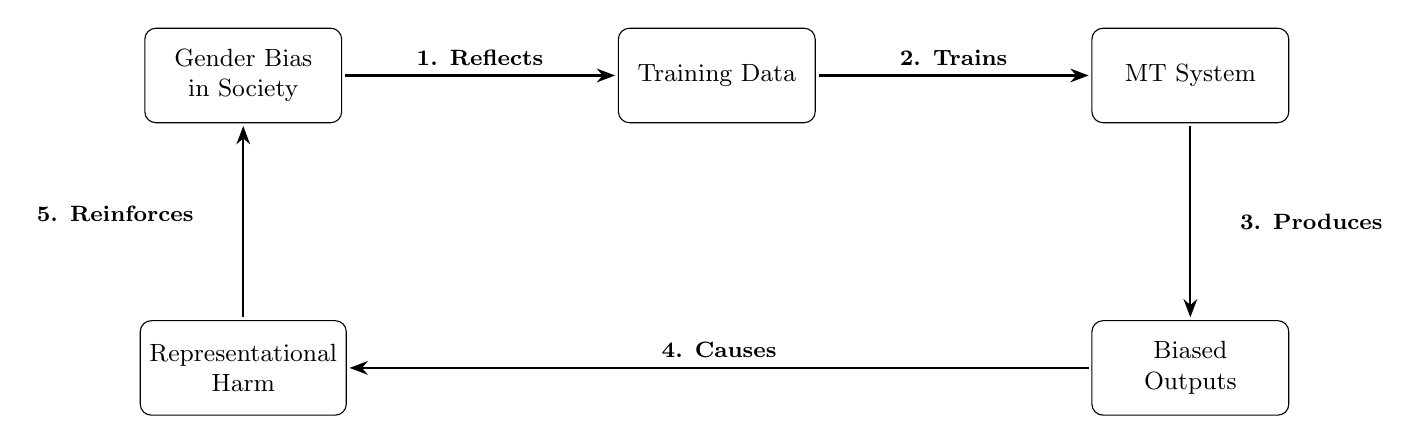
\begin{tikzpicture}[
    box/.style={rectangle, draw, rounded corners, minimum width=2.5cm, minimum height=1.2cm, align=center, font=\small},
    arrow/.style={-Stealth, thick, shorten >=1pt, shorten <=1pt},
    label/.style={midway, font=\footnotesize\bfseries}
]

\node[box] (bias) {Gender Bias\\in Society};
\node[box, right=3.5cm of bias] (data) {Training Data};
\node[box, right=3.5cm of data] (mt) {MT System};
\node[box, below=2.5cm of mt] (output) {Biased\\Outputs};
\node[box, below=2.5cm of bias] (harm) {Representational\\Harm};

\draw[arrow] (bias) -- (data) node[label, above] {1. Reflects};
\draw[arrow] (data) -- (mt) node[label, above] {2. Trains};
\draw[arrow] (mt) -- (output) node[label, right=3mm, xshift=2mm] {3. Produces};  
\draw[arrow] (output) -- (harm) node[label, above] {4. Causes};
\draw[arrow] (harm) -- (bias) node[label, left=3mm, xshift=-2mm, yshift=1mm] {5. Reinforces}; 

\end{tikzpicture}
}
            \caption{Regressive feedback loop of gender bias in MT.}
            \label{fig:regressive_feedback_loop}
        \end{figure}
        \vspace{1cm} 

        The generic masculine in particular leads to inaccurate and unfair representations of gender in translated text. \citet{rescignoGenderBiasMachine2023} observed a predominance of masculine forms in translation outputs (approximately 90\% in Google Translate and 85–88\% in DeepL for EN-IT and EN-DE), even when the original sentences contained relatively few masculine references. This shows that the bias is not minor but occurs quite heavily in those systems.

        It also contributes to the invisibility of women in male-dominated professions \citep{kapplAreAllSpanish2025}. Studies show that biased language in machine-generated text, such as children’s stories or job ads, can \textbf{influence how young people view themselves} \citep{soundararajanInvestigatingGenderBias2024,kapplAreAllSpanish2025}. It may shape their interests, hobbies, and career choices. This is especially visible in STEM fields \citep{pratesAssessingGenderBias2019}, where stereotypes are more persistent. When job descriptions or mock interviews use gender-exclusive pronouns, women report feeling less belonging, lower motivation, and weaker identification with the role \citep{godsilEffectsGenderRoles2016}. Many self-select out of applying, shrinking the female talent pool and \textbf{reinforcing gender gaps in the workforce}.

        Research also shows that using GFL like "she and he" or "one" can improve how women respond to job ads. It reduces stereotype threat and helps them engage more positively with opportunities \citep{godsilEffectsGenderRoles2016}.

        Furthermore, a study by \citet{savoldiWhatHarmQuantifying2024} measured how much effort people need to fix biased translations. They used metrics like the time it took to edit and how many edits were needed, based on human-targeted error rate. The results showed that fixing translations with feminine forms took almost twice as long and required four times more edits than those with masculine forms.

        As a result, biased translations lead to higher economic costs and a quality gap that disproportionately affects women. \citeauthor{savoldiWhatHarmQuantifying2024} argued that current automatic bias metrics miss these human impacts. They called for better evaluation methods that reflect what users actually experience.

    \subsection{Linguistic Challenges in English-German Translation}
        Although both English and German originate from the Indo-European language family \citep{baldiEnglishIndoEuropeanLanguage2008}, they have different characteristcs. English does not assign grammatical gender to nouns. The article "the" is used universally, independent of what it refers to. On the contrary, German assigns one of three grammatical gendered articles to nouns: "der" (m), "die" (f) and "das" (n). The form or ending of a noun may also change depending on its grammatical gender. While English has a few gendered word pairs, such as "actor" (m) and "actress" (f), gender distinctions in German apply broadly across the entire noun system. "Der Student" refers to a male student, whereas "die Studentin" refers to a female student. 

        Note that grammatical gender has no connection to societal or biological gender. It is a rule of the language rather than a reflection of identity. For example, the German word Mädchen (girl) is grammatically neuter and takes the article "das". This is not because the referent lacks gender, but because the suffix "-chen" automatically assigns neuter gender. Grammatical gender in German follows structural rules, even when they contradict real-world gender associations.

    \subsection{German Gender-Fair Language} \label{subsection:german_gfl}
    Gender-fair language (GFL) refers to the use of language that treats all genders equally and aims to reduce stereotyping and discrimination \citep{sczesnyCanGenderFairLanguage2016}. Three common approaches to plural mentionings in German are: 

    \begin{itemize}
        \item \textbf{Gender-neutral rewording:}  
        This uses neutral terms instead of gendered nouns, e.g., \textit{die Studierenden lernen}. A challenge for this version is that neutral alternatives do not exist for every noun and cannot be consistently applied \citep{lardelliBuildingBridgesDataset2024}.

        \item \textbf{Gender-inclusive characters:}  
        This combines masculine, feminine and non-binary forms by using a character like \textit{*}, \textit{:}, or \textit{\_}, e.g., \textit{die Student*innen lernen}. This method is consistent but may interrupt reading flow and lacks standardization \citep{lardelliBuildingBridgesDataset2024}.

        \item \textbf{Pair form:}  
        This names both gender forms, e.g., \textit{die Studentinnen und Studenten lernen}. It is currently the most used GFL form in German \citep{waldendorfWordsChangeIncrease2024}, briefly surpassing the star and colon characters as seen in \autoref{fig:gfl_types_frequency}.
    \end{itemize}

    These examples apply when the gender of the subjects is ambiguous. But when gender is known, especially in singular mentions, the generic masculine should be avoided. However, in the same way as gender bias has no clear definition, there is \textbf{no agreed standard for GFL} \citep{lardelliBuildingBridgesDataset2024, savoldiDecadeGenderBias2025}. "Fairness" therefore heavily depends on personal views, culture, and context, which raises ethical questions about debiasing systems.

    \begin{figure}
        \centering
            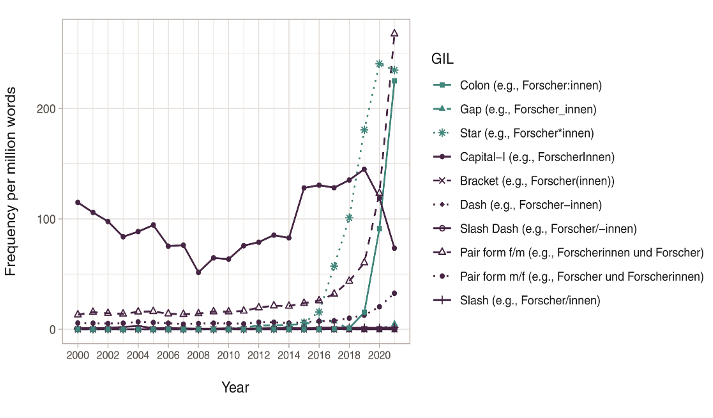
\includegraphics[width=1\textwidth]{gfl_types_frequency.png}
        \caption{Frequency of different types of gender-inclusive language. Source: \citet{waldendorfWordsChangeIncrease2024} p. 367.}
        \label{fig:gfl_types_frequency}
    \end{figure}

    \subsubsection{Challenge of Integrating Gender-Fair Language into NLP}
    Although the use of GFL has increased in recent years \citep{waldendorfWordsChangeIncrease2024}, it is still generally low. This leads to a scarcity of relevant linguistic data. Few datasets include GFL variants, and existing resources often depend on manual translations or post-editing to add gender-inclusive forms \citep{lardelliBuildingBridgesDataset2024}. For this project, the limited availability of GFL data poses a significant challenge, especially when training the model to recognize gender-fair alternatives as neutral due to the lack of consistent examples.


    % --------------------------------------------------------------------------------

    \subsection{Research Gaps}
    A central gap in gender bias research is the absence of a shared definition of what constitutes "fair" language. This lack of conceptual clarity makes it difficult to design systematic evaluation approaches, define accountability standards, or detect all relevant forms of harm \citep{barclayInvestigatingMarkersDrivers2024a,shresthaExploringGenderBiases2022,stanczakSurveyGenderBias2021}.

    A second major gap concerns the availability of high-quality EN-DE translation data that includes GFL. While a few datasets exist, they are not designed for bias detection tasks and often require manual post-editing to incorporate inclusive forms \citep{lardelliBuildingBridgesDataset2024}. This limits the development and evaluation of models that aim to identify biased output in a structured and reproducible way.

    As \citet{stanczakSurveyGenderBias2021} point out, findings on gender bias in English do not necessarily transfer to other languages such as German. This underlines the importance of typological diversity and language-specific solutions when addressing fairness in MT. Existing studies on EN-DE \citep{ullmannGenderBiasMachine2022,kapplAreAllSpanish2025,lardelliBuildingBridgesDataset2024} systems mostly confirm the presence of gender bias, propose mitigation strategies, or introduce evaluation metrics. However, few provide methods for systematically detecting bias in translated text.

    \textbf{This project addresses that gap by focusing on bias detection as a foundational step.} To support this, I combine existing datasets from previous research to create a new dataset specifically for detecting gender bias in EN-DE translations. Given the lack of suitable data and tools, detection is a necessary starting point. Manual correction will likely remain necessary, as current research does not yet support reliable automatic debiasing. This project therefore focuses on flagging biased translations, not correcting them.

% --------------------------------------------------------------------------------

\section{Approach and Justification of the Technical Setup}
This section outlines the technical setup used in the project and explains the rationale behind design choices. It also provides background information on the underlying technologies to clarify how each component contributes to the overall goal of detecting gender bias in EN-DE translations.

\subsection{Binary Classification in NLP}
    Binary classification means sorting items into two clear groups. It is the most common task in ML and is frequently found in every day life, such as automatically flitering e-mails as "spam" or "not spam" \citep{quemyBinaryClassificationUnstructured2019} or deciding whether a transaction is "fraudulent" or "legitimate". For instance, a spam filter uses previously labeled e-mails to learn relevant patterns, such as specific keywords or sender information, and builds a model that applies these patterns to classify new messages accurately. 
    
    \textbf{This thesis tries to label a translation as either "potentially gender biased" or "neutral".}. While it is possible to extend the classification beyond two categories, such as distinguishing types of bias or including labels like "gender-fair", this would require much more data and training. Given the practical aim of this work, which is to help users quickly identify whether their text might contain gender bias, the model focuses on a simple binary decision.

\subsection{Transformer Architecture} \label{subsection:transformer_arch}
Since BERT is based on the transformer architecture and is used for classification in this thesis, this section provides a brief overview of its structure. The transformer \textit{transforms} an input sequence into an output sequence, such as in translation. To effectively achieve that, they deploy a self-attention mechanism \citep{phuongFormalAlgorithmsTransformers2022}.

\subsubsection{Self-attention mechanism}
The self-attention mechanism allows the model to weigh the significance of all input elements simultaneously \citep{xiaoIntroductionTransformersNLP2023}, unlike traditional methods like Recurrent Neural Networks (RNNs), which process data sequentially. As a result, self-attention captures global dependencies and contextual relationships more accurately, creating "context-aware" representations, which is crucial for detecting subtle gender biases that depend on context within translations.

\subsubsection{Encoder-Decoder Framework} \label{subsection:encoder-decoder}
The transformer architecture consists of two main components: the encoder and the decoder. The \textbf{encoder}’s job is to read the input sentence and turn it into a series of vectors the model can understand. Each vector is a list of numbers representing the meaning and structure of each word \citep{xiaoIntroductionTransformersNLP2023}. The encoder works as follows (see \autoref{fig:transformer_architecture}):

\begin{enumerate}
    \item It receives \textbf{input embeddings}, which represent the words, and \textbf{positional encodings}, which tell the model the order of the words.
    
    \item The data then passes through several identical layers. Each layer has two main parts:
    \begin{enumerate}[label=\alph*.]
        \item \textbf{Multi-head self-attention} runs several attention processes in parallel. Each attention head focuses on different details to help the model understand the sentence better.
        \item A \textbf{Feed-forward network} processes each word vector separately, refining the information like a small filter.
        \item \textbf{Add \& Layer Norm} combines a shortcut connection (Add) and normalization (Layer Norm). The Add step passes the original input forward to keep useful information. Layer Norm adjusts the output values to a stable range so the model can learn more reliably.
    \end{enumerate}
    
    \item Each layer builds on the output of the previous one, helping the model form more complex and abstract ideas about the input sentence.
    
    \item Finally, the encoder outputs a sequence of \textit{hidden states}. These are continuous vector representations for each input token. They encode contextual information from the entire sentence. For example, in the sentence ``The cat sat on the mat,'' the vector for ``cat'' reflects its relationship to words like ``sat'' and ``mat.''
\end{enumerate}


\begin{figure}[ht]
    \centering
	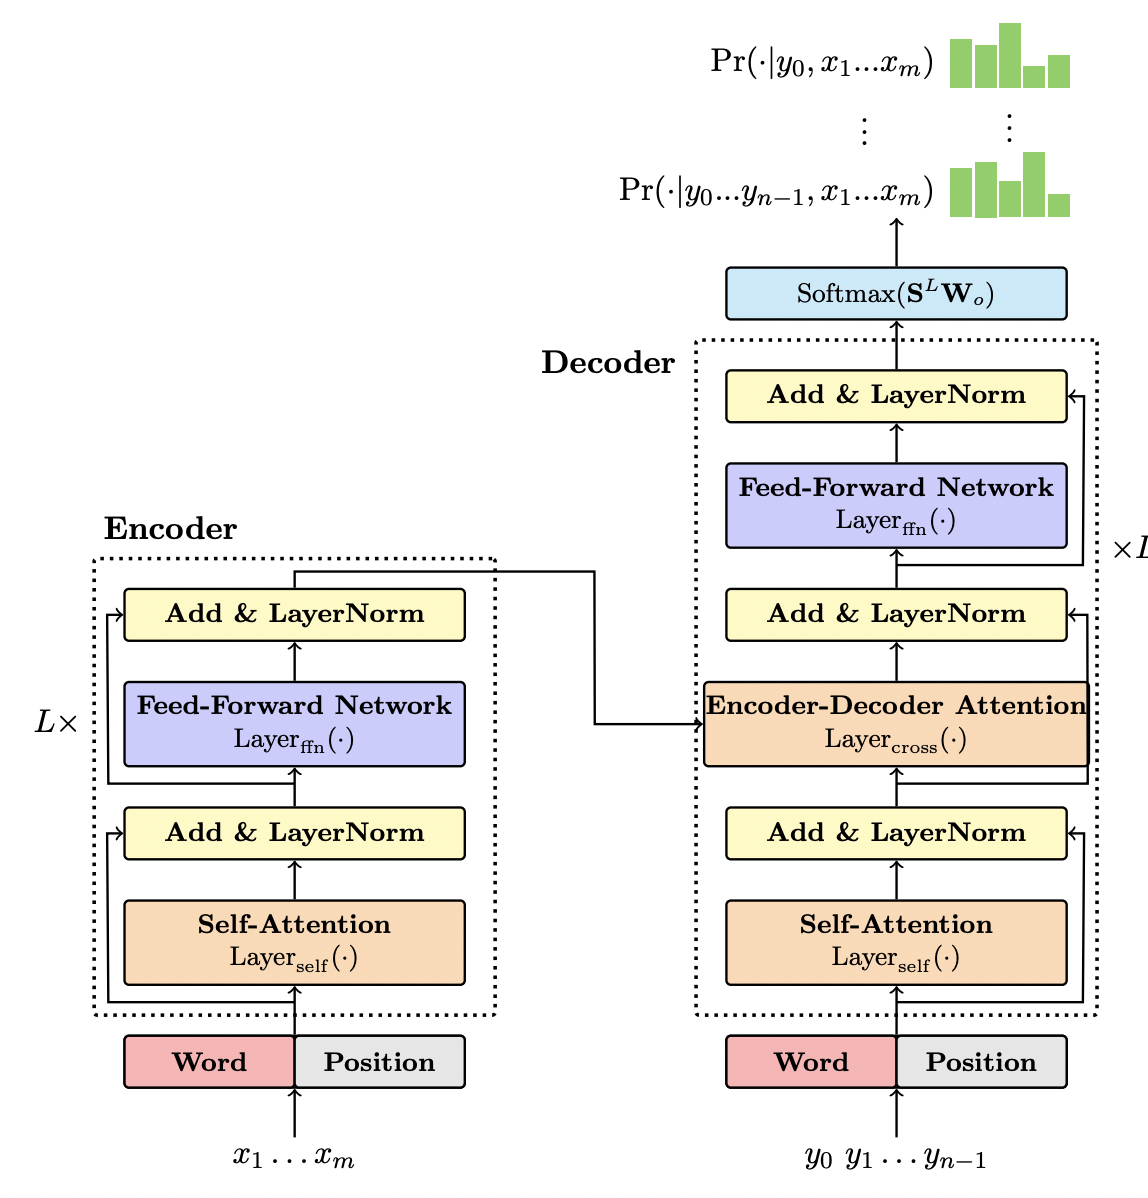
\includegraphics[width=\textwidth,height=0.45\textheight,keepaspectratio]{transformer_architecture.png}	
    \caption{Transformer encoder-decoder architecture. The encoder (left) processes input tokens \(x_1,\dots,x_m\) through: (1) a self-attention layer for contextual relationships, (2) a feed-forward network for feature transformation, and (3) residual connections with layer normalization. The decoder (right) generates outputs by attending to both the encoder's representations and its previous outputs ($y_0$ to $y_{n-1}$), producing the next-token probability distribution. Figure and description adapted from \citet{xiaoIntroductionTransformersNLP2023}, p. 6.}
    \label{fig:transformer_architecture}
\end{figure}

The \textbf{decoder} generates the output sentence one word at a time by using the information from the encode \citep{xiaoIntroductionTransformersNLP2023}. However, since BERT uses only an \textbf{encoder-only architecture}, the decoder is not relevant for this work and is therefore excluded from the discussion.

\subsection{Language model: BERT}
\emph{This entire subsection summarizes the input representation methodology from \citet{devlinBERTPretrainingDeep2019}.}

\noindent BERT is a language model that stands for "Bidirectional Encoder Representations from Transformers" and was introduced by Google in 2018 \citep{devlinBERTPretrainingDeep2019}. After pre-training, BERT can be adapted to many NLP tasks by adding a simple output layer and fine-tuning, without needing major changes to its design.

\subsubsection{Model architecture}
As explained in \autoref{subsection:transformer_arch}, BERT uses an \textbf{encoder-only architecture} (see \autoref{fig:bert_arch}). It processes and understands input thoroughly but does not generate new text. That makes BERT \textbf{well suited for binary classification tasks}, since it can analyze each word’s meaning and decide accurately between two categories.

It uses a multi-layer bidirectional Transformer encoder. Multi-layer means it stacks 12 encoder layers that refine the information step by step. Bidirectional means the model reads both the words before and after a given word at the same time. This is a key improvement over earlier models, which could only read text in one direction, usually from left to right.


\begin{figure}
    \centering
	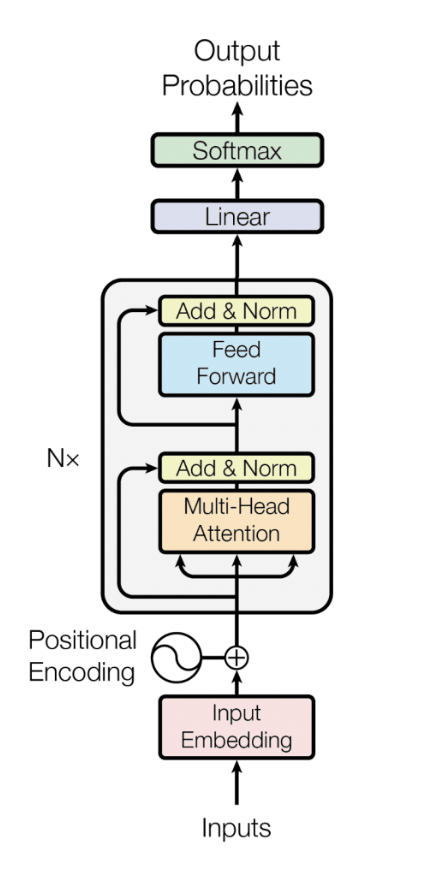
\includegraphics[width=\textwidth,height=0.4\textheight,keepaspectratio]{BERT_architecture.png}	
    \caption{BERT's encoder-only architecture. Figure by \citet{smithCompleteGuideBERT2024}.}
    \label{fig:bert_arch}
\end{figure}

\subsubsection{Input and Output Representations}
BERT processes an input by splitting whole words or subword units into \textit{tokens}. This allows the model to handle rare and compound words. For example:

\begin{quote}
    \texttt{unbelievable} $\rightarrow$ \texttt{un}, \texttt{\#\#believable}
\end{quote}

\noindent Special tokens are reserved tokens added to input sequences to indicate boundaries or roles, helping the model distinguish parts of the text and process it correctly.

\begin{itemize}
	\item \texttt{[CLS]} (classification) marks the start of the sequence,
	\item \texttt{[SEP]} separates sentence pairs.
\end{itemize}

\noindent In this work, each input combines an English source sentence and its German translation as:

\begin{quote}
    \texttt{[CLS] english sentence [SEP] german translation [SEP]}
\end{quote}

\noindent After processing, BERT outputs a hidden vector for each token. The hidden vector for the \texttt{[CLS]} token represents the entire sequence and is used for tasks like classification. For example, for the input sequence:

\begin{quote}
\texttt{[CLS] the nurse is kind [SEP] die krankenschwester ist nett [SEP]}
\end{quote}

\noindent BERT creates a vector for each token:

\[
\text{Vector}([CLS]), \text{Vector}(\text{the}), \text{Vector}(\text{nurse}), \ldots, \text{Vector}([SEP])
\]

\noindent The \texttt{[CLS]} vector aggregates the meaning of both sentences and feeds into the classifier for bias detection.


\subsubsection{Pre-training and Fine-tuning}
BERT was pre-trained on a large corpus of unlabeled text \citep{devlinBERTPretrainingDeep2019}. Since this data contains no manual labels, the model learns to understand language by using patterns in the data to learn token relationships. The result is a task-agnostic base model. In \autoref{fig:bert_arch}, this base model includes all components below the purple linear layer.\footnote{The explanation in this section is based on a prompt-response pair generated using the Perplexity.ai search engine. The original prompt and result are included as a PDF in the appendix.}

\textbf{Fine-tuning adjusts this base model for a specific task}, in this case, detecting gender bias in translations. Since this thesis focuses on the fine-tuning process, the following explanation provides more technical background for this part of the model. 

A task-specific \textbf{classification head}, comprising a linear layer followed by a softmax function, is added on top of BERT’s output. The \textbf{linear layer} applies a learned transformation to the final hidden state vector of the \texttt{[CLS]} token. 

\[
z = Wx + b
\]

Here, \(x\) is the \texttt{[CLS]} embedding, \(W\) is the weight matrix, and \(b\) is the bias vector. Both \(W\) and \(b\) are parameters learned during training to help map BERT’s output to the task labels. This changes BERT’s output into two numbers (logits), one for each class: biased or neutral. Then, \textbf{softmax} turns these numbers into probabilities:

\[
\text{softmax}(z_i) = \frac{e^{z_i}}{\sum_{j=1}^{K} e^{z_j}}
\]

Each logit \( z_i \) is exponentiated to ensure positivity. The result is then normalized by dividing by the sum of all exponentials, producing a probability distribution over the classes. \( K \) is the number of possible classes. The class with the highest probability is selected as the model’s prediction.

\subsubsection{Example: Predicting Gender Bias with Softmax}
When the model processes the sentence pair "the nurse is kind" / "die krankenschwester ist nett," it creates a \texttt{[CLS]} embedding summarizing the input. This embedding captures features such as word choice, syntactic structure, and semantic associations. 

The linear layer then transforms this embedding into two logits, for example, \([2.0, 1.0]\). The first logit corresponds to the "biased" class, and the second to "neutral". These values are not manually assigned but result from learned weights in the linear layer. During training, the model adjusts these weights to associate certain input patterns with higher scores for one class. In this case, the presence of a gendered profession ("nurse") and a feminine translation ("krankenschwester") may lead the model to assign a higher logit to the "biased" class, based on patterns seen in the training data.

To convert these logits into probabilities, the softmax function is applied:

\[
\text{softmax}([2.0, 1.0]) = \left[\frac{e^2}{e^2 + e^1}, \frac{e^1}{e^2 + e^1}\right] \approx \left[\frac{7.39}{7.39 + 2.72}, \frac{2.72}{7.39 + 2.72}\right] = [0.73, 0.27]
\]

Here, \(K=2\) because there are two classes. The model assigns a 73\% probability to the "biased" class and 27\% to "neutral". Since the "biased" probability is higher, the model predicts the translation likely contains gender bias.

\subsection{Multilingual BERT}
There are multiple variants of the original BERT model. Even the standard version was released in two sizes: BERT-Base and BERT-Large, which differ in the number of layers, attention heads, and overall model capacity \citep{devlinBERTPretrainingDeep2019}. Since then, many other versions have been developed. Most of them modify either BERT’s pre-training objectives or the underlying Transformer architecture \citep{libovickyHowLanguageNeutralMultilingual2019}.

For this thesis, I use multilingual BERT \textbf{\href{https://huggingface.co/google-bert/bert-base-multilingual-cased}{(mBERT)}} \citep{devlinBERTPretrainingDeep2019}. mBERT uses the same configuration as BERT-Base, but it is pretrained on Wikipedia data from 104 languages, including both English and German. There is no explicit indication of the input language, nor is there a training objective that aligns languages bilingually; instead, multilingual capabilities emerge naturally from training on a large multilingual text corpus \citep{piresHowMultilingualMultilingual2019}.

Monolingual models like \href{https://huggingface.co/google-bert/bert-base-german-cased}{German BERT} do not support English input. Larger multilingual models, such as \href{https://huggingface.co/docs/transformers/en/model_doc/xlm-roberta}{XLM-RoBERTa}, require more computational resources and training time, which was not feasible here. mBERT offers a good balance between language coverage, model size, and training efficiency, making it a practical choice detecting gender bias in EN-DE translations.

\subsection{Interactive Demo}
The fine-tuned model is intended to be presented through an interactive demonstration. Since the focus lies on showcasing the model’s functionality rather than creating a fully developed application, \href{https://streamlit.io/}{Streamlit} was chosen. Streamlit allows for quick and easy development of lightweight user interfaces in Python, providing a simple setup and effective performance.

For live translation, an open-source tool supporting EN-DE pairs was required. \href{https://github.com/Helsinki-NLP/Opus-MT}{Opus-MT} \citep{tiedemannOPUSMTBuildingOpen2020} meets these criteria and integrates smoothly into the demonstration. While state-of-the-art translators like Google Translate or DeepL would have been preferred for their quality, they do not meet the requirements for this setup. Therefore, a separate tab for manual translation input was added, allowing users to paste translations directly and bypass this limitation.
    \clearpage{\pagestyle{empty}\cleardoublepage}		
    \chapter{Methodology}
The goal of this project is to develop a practical gender bias detection model tailored for real-world MT scenarios. It targets common use cases like translating everyday sentences or job descriptions, focusing on flagging biased language at the sentence level. This means the model evaluates each sentence independently, without considering context from surrounding sentences. This approach guides both the model’s design and the preparation of the training data, where each translation pair is treated as a separate example. The project begins by selecting and combining datasets from previous work (see \autoref{fig:workflow}). The model building phase then follows, as shown in the purple boxes. It starts with cleaning and preparing the data, followed by extracting features for training. A pre-trained \texttt{mBERT} model is then fine-tuned for the classification task. Its performance is measured using standard evaluation metrics. In the final step, the trained model is integrated  into the demo application.

\vspace{1cm} 
\begin{figure}[htb]
    \centering
    \scalebox{0.8}{\tikzstyle{startstop} = [rectangle, rounded corners, minimum width=3cm, minimum height=1cm,text centered, draw=black, fill=gray!20]
\tikzstyle{process} = [rectangle, minimum width=3cm, minimum height=1cm, text centered, draw=black, fill=blue!10]
\tikzstyle{arrow} = [thick,->,>=stealth]

\begin{tikzpicture}[node distance=1.7cm]

\node (start) [startstop] {Select and Combine Datasets};
\node (clean) [process, below of=start] {Clean and Pre-process Data};
\node (features) [process, below of=clean] {Extract Features};
\node (train) [process, below of=features] {Train Model};
\node (evaluate) [process, below of=train] {Evaluate Model Performance};
\node (demo) [startstop, below of=evaluate] {Show Model in Demo Application};

\draw [arrow] (start) -- (clean);
\draw [arrow] (clean) -- (features);
\draw [arrow] (features) -- (train);
\draw [arrow] (train) -- (evaluate);
\draw [arrow] (evaluate) -- (demo);

\end{tikzpicture}
}
    \caption{Methodology Overview}
    \label{fig:workflow}
\end{figure}
\vspace{1cm} 

\section{Dataset}
    Since no ready-to-use dataset existed for this task and no prior work had developed a comparable model, it was necessary to define: \textbf{(1)} the required number of samples, and \textbf{(2)} the desired content of the dataset. For a binary classification task of detecting gender bias using \texttt{mBERT}, general guidelines suggest between 100 and 5,000 labeled samples for fine-tuning \parencite{pecherComparingSpecialisedSmall2024}, while multi-class tasks need fewer samples (around 100). However, the complex nature of gender bias often requires a larger dataset for robust detection since the number of samples depends mainly on the task type. For the final dataset, 2,000 to 5,000 samples were selected to provide enough data for effective training while staying within resource limits.

    Existing EN-DE datasets were reviewed to reduce the need for manual data creation. The following sources were considered: \texttt{\href{https://huggingface.co/datasets/FBK-MT/mGeNTE}{mGeNTE en-de}} \parencite{savoldiMGeNTEMultilingualResource2025}, \texttt{\href{https://github.com/g8a9/building-bridges-gender-fair-german-mt}{Building Bridges Dictionary}} \parencite{lardelliBuildingBridgesDataset2024}, and \texttt{\href{https://research.google/blog/a-dataset-for-studying-gender-bias-in-translation/}{Translated Wikipedia Biographies}} \parencite{stellaDatasetStudyingGender2021}.

    Analysis of the \texttt{Translated Wikipedia Biographies} dataset revealed several issues that prevented direct reuse. In many instances, the \texttt{perceivedGender} column contained subject names instead of expected labels such as \texttt{Male}, \texttt{Female}, or \texttt{Neutral}, making manual verification necessary. Additionally, all examples were labeled as neutral (0), as the dataset was designed around correctly gendered references. Since the remaining two datasets were already balanced and contained a sufficient number of neutrally gendered examples, the Wikipedia Biographies dataset was excluded from the final training data. \texttt{mGeNTE} contains naturally occurring sentences with gendered entities, while \texttt{Building Bridges} focuses on German GFL entries for explicitly gendered nouns such as professions. 

\begin{table}[ht!]
    \centering
    \renewcommand{\arraystretch}{1.3}
    \begin{tabularx}{\textwidth}{|>{\raggedright\arraybackslash}X|>{\raggedright\arraybackslash}X|>{\raggedright\arraybackslash}X|}
    \hline
    \textbf{Dataset} & \textbf{Description} & \textbf{Content} \\ \hline
    \texttt{mGeNTE en-de} \parencite{savoldiMGeNTEMultilingualResource2025} & Multilingual dataset to assess gender bias in MT. & \textasciitilde1,500 gender-ambiguous and gendered English sentences with gender-neutral and gendered German translations. \\ \hline
    \texttt{Building Bridges Dictionary} \parencite{lardelliBuildingBridgesDataset2024} & Bilingual dictionary designed to support gender-fair EN-DE translation. & \textasciitilde230 German gender-neutral and gender-inclusive singular and plural sentences with English equivalents. \\ \hline
    \end{tabularx}
    \caption{Overview of suitable EN-DE datasets based on past works}
    \label{tab:available_datasets}
\end{table}

\subsection{Pre-processing}

\subsubsection{mGeNTE en-de} 
The mGeNTE dataset contained the following relevant information:  

\begin{itemize}  
  \item \texttt{SET-G}: English sentences with a clearly gendered subject.  
  \item \texttt{SET-N}: English sentences with neutral or ambiguous subject gender.  
  \item \texttt{REF-G}: German translations that preserve or introduce gender.  
  \item \texttt{REF-N}: German translations that are fully gender–neutral.  
\end{itemize}  

\noindent
The bias definition used in this study classifies translations that omit the original gender as neutral, as they do not rely on a male default or stereotype. Although gender-neutral translations may be imperfect, they are not considered biased within this framework. Initial experiments indicated that including \texttt{REF-N} pairs during training led to over-penalization of neutral outputs. Due to the limited availability of neutral examples, such outputs were not penalized in the final training setup. Each original entry was split into two paired examples and labeled as follows:  
\[
\begin{aligned}
\texttt{SET\!-\!G} + \texttt{REF\!-\!G} &\;\rightarrow\; 0 \quad(\text{neutral})\\
\texttt{SET\!-\!G} + \texttt{REF\!-\!N} &\;\rightarrow\; 0 \quad(\text{neutral})\\
\texttt{SET\!-\!N} + \texttt{REF\!-\!N} &\;\rightarrow\; 0 \quad(\text{neutral})\\
\texttt{SET\!-\!N} + \texttt{REF\!-\!G} &\;\rightarrow\; 1 \quad(\text{biased})
\end{aligned}
\]  
This procedure yields 3,000 total instances, of which 750 are labeled biased (1) and 2,250 are labeled neutral (0).\footnote{The transformed dataset can be found in \texttt{/datasets/mgente\_final.csv}.} 

\subsubsection{Building Bridges Dictionary} 
This dataset consisted of a GFL dictionary of nouns, not full sentences. That made it useful for studying GFL, but not suitable for this task, which requires sentence-level context. To address this, prompt engineering was used with Google Gemini 2.5 Flash to synthetically expand the dataset. The prompt is included in the appendix; the generated sentences are available in the code files. Nouns from the original dataset were used to create multiple grammatically correct sentence variations, covering singular, plural, gender-neutral, and gender-inclusive forms. The dataset uses the star form (e.g., \textit{Lehrer*innen}) as its inclusive format. Since the colon form (e.g., \textit{Lehrer:innen}) is also common in practice, a script was used to duplicate all entries with stars and replace the star with a colon to generate additional variants. This resulted in 3,381 total entries: 2,001 labeled as 0 (neutral) and 1,380 labeled as 1 (biased).\footnote{The transformed dataset can be found in \texttt{/datasets/lardelli\_final.csv}.}

\subsubsection{Tatoeba} 

The aforementioned setup lacked genuinely neutral examples, defined as sentences without any gendered subject, such as "The weather is nice" or "How are you". Including such cases is important for training the model to recognise that not all translations are relevant for gender bias detection, and that many sentences should be classified as neutral. As no suitable dataset for this category was available, a supplementary set was created from random EN–DE sentence pairs drawn from the \texttt{\href{https://tatoeba.org/en/}{Tatoeba}} corpus. A total of 550 sentence pairs was sampled. Manual filtering was applied to remove any pairs containing incorrect translations or stereotypical gendering, as public contributions often default to male forms. The final subset contained 532 clearly neutral sentence pairs, all labelled with 0.\footnote{The transformed dataset can be found in \texttt{/datasets/tatoeba\_final.csv}.}


\subsubsection{Available Data Summary}

\autoref{tab:data-summary} shows an overview of the labeled data from the three available sources. 

\begin{table}[H]
\centering
\begin{tabularx}{\textwidth}{l *{3}{>{\centering\arraybackslash}X}}
\toprule
\textbf{Dataset} & \textbf{Total} & \textbf{Neutral (0)} & \textbf{Biased (1)} \\
\midrule
\texttt{lardelli\_final.csv} & 3381 & 2001 & 1380 \\
\texttt{mgente\_final.csv}   & 3000 & 2250 & 750  \\
\texttt{tatoeba\_final.csv}      & 532  & 532  & 0    \\
\bottomrule
\end{tabularx}
\caption{Summary of available labeled examples}
\label{tab:data-summary}
\end{table}

The number of samples selected from each dataset was determined through iterative testing. Multiple dataset variants were created by upsampling or downsampling specific groups. The documentation of this process is discussed in \autoref{subsection:hyperparameter_tuning_methodology}.

\subsection{Data Splitting and Cleaning}
    The dataset is partitioned into training (80\%), validation (10\%), and test (10\%) subsets. This splitting ratio follows established practices commonly employed in ML experiments \parencite{bahetiTrainTestValidation2021}. It provides enough samples for the model to learn general patterns while reserving separate subsets for tuning and final evaluation. Stratified sampling was used to maintain consistent label distribution (biased vs. neutral) across all three sets. For example, if 30\% of the full dataset is biased, each split will also have 30\% biased samples. 

    Advanced text cleaning steps (punctuation removal, lowercasing, or stemming) were not applied due to the use of \href{https://huggingface.co/google-bert/bert-base-multilingual-cased}{\texttt{bert-base-multilingual-cased}}. This tokenizer handles raw, unaltered text and retains case distinctions. The model was pretrained on large corpora containing natural language in its original form \parencite{devlinBERTPretrainingDeep2019}, so modifying the input by lowercasing or stripping punctuation could remove meaningful patterns the model has learned to recognize. Steps to handle missing values or invalid entries were already performed in the individual datasets, so they did not need to be repeated when creating the final merged dataset.

\section{Training Pipeline}
    \texttt{mBERT} with a binary classification head is used to predict whether a translation is \textit{biased} or \textit{neutral}. The tokenizer encodes input sentence pairs into numerical representations and distinguishes between source and target sentences. All sequences are padded or truncated to a fixed length of 256 tokens, which preserves most content while keeping processing efficient. The model represents each input pair with a summary vector of the entire sequence, which is then used for classification into the two categories. Each dataset is instantiated and encoded into a format suitable for model input, including the EN–DE sentence pairs and their corresponding labels. Training hyperparameters are established through tuning. The model iteratively learns from the training data by adjusting its parameters to minimize classification errors, with validation performance guiding the process and helping prevent overfitting. At the end of training, the best-performing model is selected based on validation metrics and used for subsequent gender bias detection.

\section{Evaluation Strategy}
    Model evaluation was performed during training using the validation set and after training using two distinct test sets. As detailed in \autoref{subsection:hyperparameters_explained}, the macro F1 score was employed as the primary metric to assess model performance. The validation set served to monitor training progress across epochs, and the checkpoint with the highest validation F1 score was saved. The combined training dataset was handcrafted and had known limitations, so relying solely on the validation set was insufficient to assess final model performance. To better evaluate generalization, a separate handcrafted test set was created. This set contains EN-DE sentence pairs with manually assigned bias labels. Using these two evaluation strategies, both the fine-tuning process and the composition of the combined training dataset were iteratively adjusted to improve model robustness and generalization.

\subsection{Handcrafted Test Set Construction} \label{subsection:eval_dataset}
    The handcrafted test set was developed from a user-centered perspective, focusing on identifying inputs that expose various failure and edge cases. Examples were organized into categories: neutral sentences, neutral sentences containing gendered roles, biased translations, and translations featuring German GFL. It comprises simple synthetic sentences written specifically for this purpose, as well as authentic examples extracted from job postings. The inclusion of real-world data aims to simulate practical use cases, such as evaluating translated job advertisements for gender bias.

    Emphasis was placed on diversity in sentence structure and content rather than maintaining label balance. Certain examples tested the model’s tendency to incorrectly flag neutral sentences containing gendered terms, while others assessed its capacity to detect various GFL forms in German, including terms like “Lehrende” and the colon notation “Lehrer:innen.” Bias labels were assigned manually according to the criteria established in Chapter 2. The complete handcrafted test set, containing 26 labeled translation pairs, is provided in the Appendix.

\subsection{Hyperparameter Selection and Tuning} \label{subsection:hyperparameter_tuning_methodology}
     While a few standard hyperparameters were tested, the focus was placed on tuning dataset composition and the number of frozen layers. These factors showed a significantly stronger influence on model performance during experimentation. Since the training data originated from a mix of external sources with varying quality, adjusting the use and structure of the data was considered more effective than extensive hyperparameter optimization. Recommended default values from prior work provided sufficiently strong baselines and were therefore used as the starting point.

    \paragraph{Epochs} The model was trained for a maximum of 8 epochs, with early stopping enabled using a patience of two epochs. This setup halted training if the macro F1 score did not improve over two consecutive epochs. The approach follows the recommendation by \textcite{pecherComparingSpecialisedSmall2024}, who suggest training until convergence, with a cap of 10 epochs and early stopping. In this case, validation loss typically increased after 8 epochs, with no further improvements observed. Limiting the training to 8 epochs helped mitigate overfitting and reduced training time.

    \paragraph{Batch size} A batch size of 16 was used. This value is commonly applied in fine-tuning scenarios involving small datasets, offering a reasonable balance between memory efficiency and training stability. Smaller batch sizes paired with lower learning rates were tested but led to reduced performance and less effective learning in early epochs. Existing literature, including \textcite{mosbachStabilityFinetuningBERT2021}, supports the use of a batch size of 16; no further experiments with smaller values were conducted.

    \paragraph{Learning rate} The learning rate was set to 2e-5. This value, originally proposed in \textcite{devlinBERTPretrainingDeep2019}, remains widely used for fine-tuning transformer models. Alternatives such as 1e-5 and 3e-5 were evaluated but yielded slightly lower validation scores. The 2e-5 setting showed the most stable and consistent results and was therefore applied in all final training runs.

    \paragraph{Optimizer and scheduler} The \texttt{Trainer} API employed the AdamW optimizer by default. A warmup-linear learning rate schedule was used: the rate gradually increased during the first 10\% of training steps (warmup) and then decreased linearly until completion. This schedule supports smooth learning and helps prevent instability during early training.

\subsection{Training Dataset Tuning} \label{subsection:training_dataset_tuning}
    Since the F1 scores were similar across dataset versions, the main evaluation was based on the handcrafted test set of 25 sentences.\footnote{The detailed documentation of each iteration is included in the appendix. The focus in this section is on the process and rationale rather than on numeric results.} This small test set does not provide a complete indication of overall model quality, but it offers insight into practical usability. Any statements regarding better or worse performance should be considered in light of this limitation.

    The dataset \texttt{mgente\_final} was considered the best source because its samples are natural sentences. All 750 biased samples from \texttt{mgente\_final} were included, along with exactly 750 neutral samples. The tuning process aimed to adjust the remaining datasets to maintain a maximum ratio of 60\% neutral to 40\% biased samples. Sampling was performed using the \texttt{join\_datasets.py} script, which loads the labeled datasets, samples a fixed number of biased and neutral entries per dataset using a fixed random seed (10), and combines them into a single training set. The script also checks for missing values and label integrity before saving the final CSV file. The tuning process across dataset versions, including their composition and rationale, is summarized in \autoref{tab:dataset_versions}.

    The Baseline dataset already achieved strong performance, with a test F1 score of 0.975 and 84.6\% accuracy on the handcrafted test set. However, it failed on some neutral examples such as \textit{"My mother is an engineer." / "Meine Mutter ist Ingenieurin."} (predicted biased with confidence 0.55) and on certain German GFL patterns (e.g., double naming and the colon notation). Adjustments made to the dataset composition in Datasets B through E occasionally improved specific weaknesses. In one case, Dataset E succeeded in correctly classifying a neutral gendered sentence that the Baseline had misclassified. At the same time, these targeted improvements often introduced new issues, such as misclassifications in job advertisement examples. The changes did not produce consistent gains on the handcrafted test set and in some cases reduced overall accuracy. As a result, the Baseline dataset composition was used for final training, as it offered the most reliable balance between targeted performance and general usability.

\vspace{0.8em}
\begin{table}[ht]
    \centering
        \begin{tabularx}{\textwidth}{l X >{\raggedright\arraybackslash}X}
    \toprule
    \textbf{Dataset} & \textbf{Rationale} & \textbf{Sample Distribution (biased/neutral)} \\
    \midrule
    A & Initial setup using equal parts of \texttt{mgente\_final} and \texttt{lardelli\_final}, with some \texttt{tatoeba\_final} neutrals. & mgente 750 / 750, lardelli 750 / 750, tatoeba 0 / 250 \\
    B & Built on A. Increased \texttt{lardelli\_final} neutrals to better capture GFL patterns and added more \texttt{tatoeba\_final} neutrals. & mgente 750 / 750, lardelli 750 / 1000, tatoeba 0 / 400 \\
    C & Built on A and B. Reduced \texttt{lardelli\_final} biased examples to counter possible overrepresentation. & mgente 750 / 750, lardelli 400 / 750, tatoeba 0 / 250 \\
    D & Built on A and C. Further improved neutral recognition by adding more \texttt{tatoeba\_final} neutral sentences. & mgente 750 / 750, lardelli 750 / 750, tatoeba 0 / 500 \\
    E & Built on A and C. Increased \texttt{mgente\_final} neutral data to raise diversity from naturalistic examples. & mgente 750 / 1,250, lardelli 750 / 750, tatoeba 0 / 250 \\
    \bottomrule
    \end{tabularx}
    \caption[Dataset iterations with rationale and composition]{Dataset iterations with rationale and composition. Each version builds on the Baseline and previous adjustments. Format: source biased / neutral}
    \label{tab:dataset_versions}
\end{table}


\subsection{Layer Freezing Tuning}
    All dataset tuning experiments described above were conducted with layer freezing set to $n=8$, meaning that encoder layers 0 through 7 of \texttt{mBERT} were frozen during training. As explained in \autoref{subsection:hyperparameters_explained}, earlier studies have shown that the middle layers are most semantically informative, while lower layers tend to capture syntactic information. Freezing up to layer 8 was chosen as a baseline to reduce training time while still allowing the model to adapt higher-level representations to the task.Since the results with $n=8$ were already promising, only two further variations were tested: $n=7$ and $n=6$. These settings freeze fewer layers, meaning more of the network remains trainable. The purpose of these tests was to evaluate whether this added flexibility improved performance without overfitting.

    \vspace{0.8em}
    \begin{table}[ht]
        \centering
        \begin{tabularx}{\linewidth}{Xcc}
        \toprule
        \textbf{Frozen Layers} & \textbf{Test F1 (weighted)} & \textbf{Handcrafted Test Set Accuracy} \\
        \midrule
        $n=6$ (layers 0--5 frozen) & 0.981 & 80.8\% \\
        $n=7$ (layers 0--6 frozen) & 0.979 & 80.8\% \\
        $n=8$ (layers 0--7 frozen) & 0.966 & 84.8\% \\
        \bottomrule
        \end{tabularx}
        \caption{Comparison of layer freezing settings}
    \end{table}

    Freezing fewer layers led to slightly higher F1 scores on the test set, but the model with $n=8$ frozen layers achieved the best results on the handcrafted test sentences, which were designed to reflect real-world usability. Since the F1 differences were minor and freezing more layers results in a simpler and more efficient model, $n=8$ was chosen as the final setting.

\section{Demo Application Design}
    The demo application comprises three modules: the user interface, the bias detection model, and the translation component (see \autoref{fig:demo_workflow}). Both input modes converge on a common prediction pipeline. On launch, the application loads the trained model and its encoding mechanism into memory. Users can either input raw English text, which is split into sentences and translated into German, or provide aligned EN-DE sentence pairs. Both approaches result in a set of sentence pairs ready for bias analysis. The bias detection pipeline processes these sentence pairs by converting each pair into a representation suitable for the model. The model then predicts whether a translation is biased or neutral. Predictions are accompanied by a confidence score, which is the probability assigned by mBERT to the predicted label. Results are displayed alongside the original and translated sentences. If bias is detected above a defined threshold, a warning is shown; otherwise, the sentence pair is marked as neutral. Each result is separated to maintain readability.

    The interface has two main modes. In automatic translation, raw English text is submitted, segmented into sentences, and translated. Each sentence is paired with its translation before analysis. In manual pairing, users provide EN-DE sentence pairs directly, which bypasses translation and proceeds to bias evaluation. The system is designed to demonstrate the end-to-end process of bias detection independently of implementation details. The methodology allows the translation component or model representation to be replaced with alternative approaches. The focus is on showing how input sentences are converted into pairs, analyzed for bias, and presented in a user-friendly way. 

    \begin{figure}[htb]
    \centering
    \scalebox{0.8}{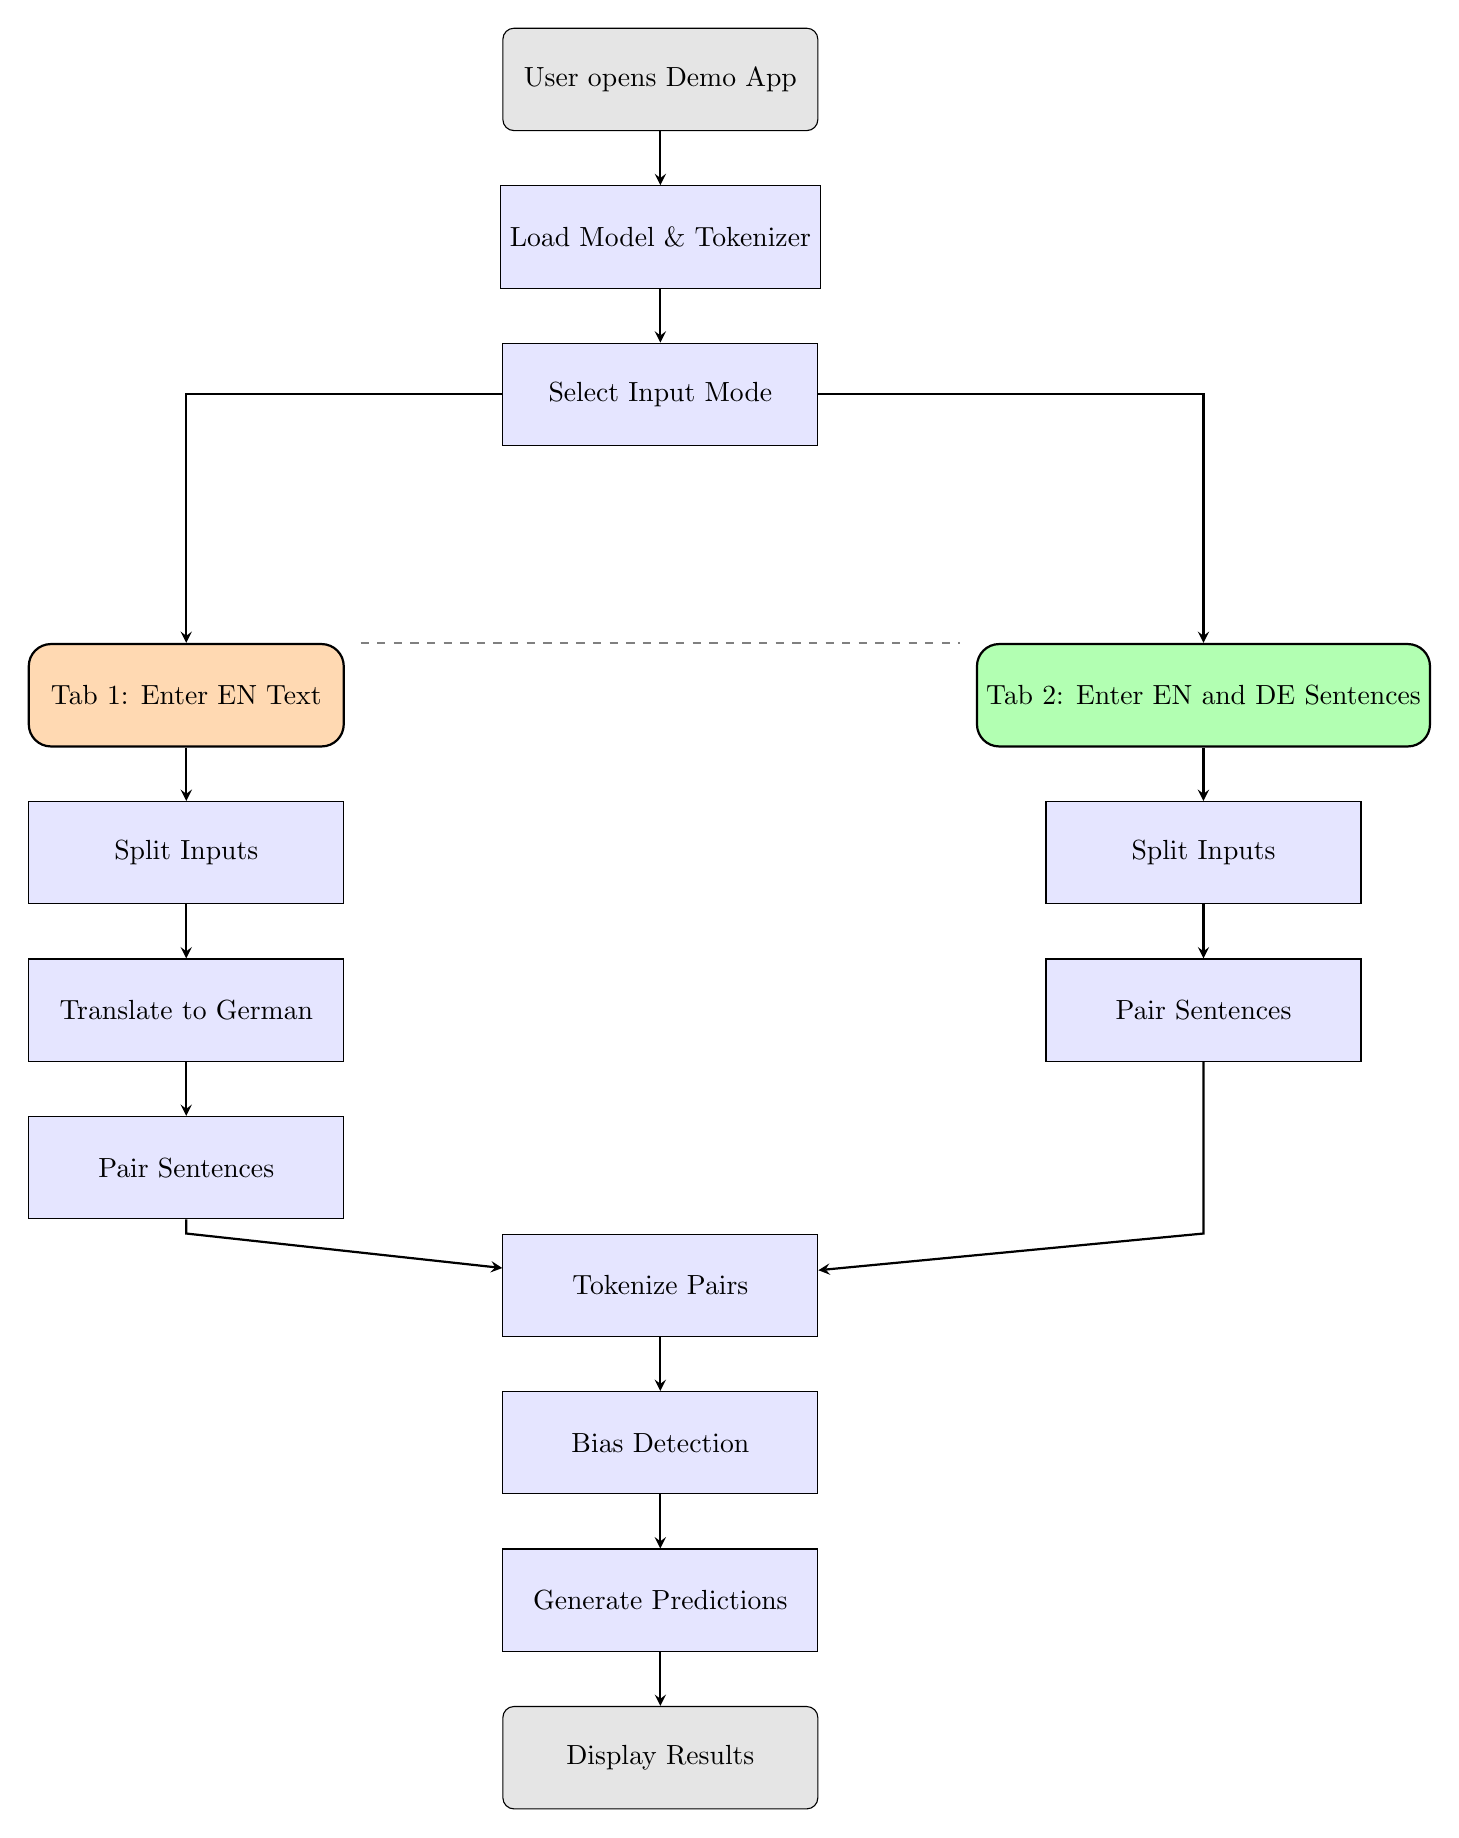
\begin{tikzpicture}[
    node distance=2cm, 
    every node/.style={font=\normalsize},
    startstop/.style={
        rectangle, 
        rounded corners, 
        minimum width=4cm, 
        minimum height=1.3cm, 
        text centered, 
        draw=black, 
        fill=gray!20
    },
    process/.style={
        rectangle, 
        minimum width=4cm, 
        minimum height=1.3cm, 
        text centered, 
        draw=black, 
        fill=blue!10
    },
    tab/.style={
        rectangle, 
        rounded corners=8pt, 
        minimum width=4cm, 
        minimum height=1.3cm, 
        text centered, 
        draw=black, 
        fill=orange!30,
        thick
    },
    arrow/.style={
        thick,
        ->,
        >=stealth
    }
]

% Start
\node (start) [startstop] {User opens Demo App};

% Model Loading
\node (load) [process, below of=start] {Load Model \& Tokenizer};

% Tabs
\node (tabs) [process, below of=load] {Select Input Mode};

% Tab 1 flow (left branch)
\node (tab1) [tab, below left=2.5cm and 2cm of tabs] {Tab 1: Enter EN Text};
\node (split1) [process, below of=tab1] {Split Inputs};
\node (translate) [process, below of=split1] {Translate to German};
\node (pair1) [process, below of=translate] {Pair Sentences};

% Tab 2 flow (right branch)
\node (tab2) [tab, below right=2.5cm and 2cm of tabs, fill=green!30] {Tab 2: Enter EN and DE Sentences};
\node (split2) [process, below of=tab2] {Split Inputs};
\node (pair2) [process, below of=split2] {Pair Sentences};

% Common processing - positioned lower to accommodate 90-degree arrows
\node (tokenize) [process, below=10cm of tabs] {Tokenize Pairs};
\node (predict) [process, below of=tokenize] {Bias Detection};
\node (results) [process, below of=predict] {Generate Predictions};
\node (display) [startstop, below of=results] {Display Results};

% Arrows - Main flow
\draw [arrow] (start) -- (load);
\draw [arrow] (load) -- (tabs);
\draw [arrow] (tabs) -| (tab1);
\draw [arrow] (tabs) -| (tab2);

% Arrows - Left branch
\draw [arrow] (tab1) -- (split1);
\draw [arrow] (split1) -- (translate);
\draw [arrow] (translate) -- (pair1);
\draw [arrow] (pair1) -- (pair1 |- tokenize.north) -- (tokenize);

% Arrows - Right branch
\draw [arrow] (tab2) -- (split2);
\draw [arrow] (split2) -- (pair2);
\draw [arrow] (pair2) -- (pair2 |- tokenize.north) -- (tokenize);

% Arrows - Common processing
\draw [arrow] (tokenize) -- (predict);
\draw [arrow] (predict) -- (results);
\draw [arrow] (results) -- (display);

% Dashed line to show parallel flows
\draw [dashed, gray] ($(tab1.north east)+(0.2,0)$) -- ($(tab2.north west)-(0.2,0)$);

\end{tikzpicture}
}
    \caption[Process of the bias detection application]{Process of the bias detection application. Automatic translation and manual sentence pairs follow the same prediction steps}
    \label{fig:demo_workflow}
\end{figure}

    \clearpage{\pagestyle{empty}\cleardoublepage}		
    \chapter{Implementation}
Based on the methodology, this chapter presents the specific implementation carried out in this project, along with step-by-step instructions to run the demo and reproduce the results. The complete project repository, including all datasets and scripts, is available at \url{https://github.com/phmkhali/bias-detector-en-de}.

\section{Environment Setup and Project Structure}
    \subsection{System Environment and Hardware}
    The project was developed on macOS using Python 3.12.4. A virtual environment was used, and all dependencies were installed via the \texttt{requirements.txt} file using \texttt{pip3}. No manual installation steps were needed beyond this. During development, both GPU and CPU were used to test training and inference performance, with device selection handled dynamically. The final model for the demo and evaluation was trained on the CPU to ensure full compatibility and reproducibility without relying on a GPU. To ensure reproducibility, random seeds were fixed across all libraries and backends. The application is started via Streamlit. Further usage instructions are provided in \autoref{section:reproduction_guide}.

\subsection{Directory Layout}
    \autoref{fig:file_tree} shows the directory structure with the relevant files for the final implementation. The folder contains additional files related to the original datasets and scripts used for data conversion. These supplementary files are intended for comprehension and reproducibility purposes but are not required for the final model.

    \vspace{0.8em} 
    \begin{figure}[htb]
        \centering
        \scalebox{0.8}{\begin{forest}
  for tree={
    font=\ttfamily,
    grow'=0,
    child anchor=west,
    parent anchor=south,
    anchor=west,
    calign=first,
    edge path={
      \noexpand\path [draw, \forestoption{edge}]
      (!u.south west) +(7.5pt,0) |- (.child anchor) \forestoption{edge label};
    },
    before typesetting nodes={
      if n=1
        {insert before={[,phantom]}}
        {}
    },
    fit=band,
    before computing xy={l=15pt},
  }
[bias-detector-en-de
    [datasets
      [dataset.csv]
      [join\_datasets.py]
      [lardelli\_final.csv]
      [mgente\_final.csv]
      [tatoeba\_final.csv]
    ]
    [model\_output]
    [app.py]
    [fine-tuning.ipynb]
    [translate.py]
    [utils.py]
  ]
\end{forest}

}
        \caption[Relevant files of the final implementation]{Relevant files of the final implementation}
        \label{fig:file_tree}
    \end{figure}
    \vspace{0.8em} 


\section{Core Components and Data Flow}
    \subsection{Datasets Folder}
        The \texttt{datasets} folder contains the processed datasets used for training and evaluation of the bias detection model. It includes the final combined dataset \texttt{dataset.csv} as well as intermediate datasets derived from individual sources: \texttt{lardelli\_final}, \texttt{mgente\_final}, and \texttt{tatoeba\_final}. The \texttt{join\_datasets} script facilitates the concatenation of these datasets into a unified dataset. The script is designed to support iterative sampling by specifying sample sizes for biased and neutral classes with a fixed random seed. It merges the sampled subsets, shuffles the combined data, and performs data integrity checks. 

    \subsection{Fine-tuning Notebook and Model Output}
        The \texttt{fine-tuning.ipynb} notebook carries out the complete process of preparing and fine-tuning the bias detection model. It begins by loading the pretrained \texttt{mBERT} model and the training dataset (\texttt{dataset.csv}). Each dataset is instantiated using a custom \texttt{BiasDataset} class, which encodes EN-DE sentence pairs and their labels into tensors suitable for model input. Training configurations are defined via \texttt{TrainingArguments}, specifying evaluation intervals and checkpoint saving strategies. A \texttt{Trainer} object is then created with the model, datasets, training arguments, and a metric computation function.

        The training proceeds by feeding batches from the training dataset to the model, updating the weights based on the loss, and evaluating performance on the validation set at the end of each epoch. Early stopping limited the process to six epochs, taking approximately 18 minutes and 32 seconds on the development machine. Checkpoints, configuration files, tokenizer files, and training metadata are saved in the \texttt{model\_output} folder, with the best-performing model retained for subsequent use in bias detection.

    \subsection{Streamlit Application}
        The \texttt{app.py} file is the main entry point for the Streamlit interface.\footnote{Parts of the code were generated with AI and subsequently refined by the author; see Appendix \ref{appendix:ai_code} for details.}
        It loads the fine-tuned model and tokenizer from the \texttt{model\_output} directory and sets up the classification pipeline. In the automatic tab, users enter English text, which is translated using \texttt{translate.py}. In the manual tab, users enter both the original and translated sentences directly.\footnote{Screenshots of these tabs are shown in Figures~\ref{fig:demo_tab_1}, \ref{fig:demo_tab_2}, and \ref{fig:demo_multi_sentence}.} \texttt{translate.py} wraps the pre-trained OpusMT EN-DE model from Hugging Face. The main function, \texttt{translate\_batch}, takes a list of English sentences, tokenizes them, and uses the model's \texttt{generate} method to return a list of decoded German translations. The resulting sentence pairs from both tabs are passed to functions in \texttt{utils.py}. This module handles sentence splitting, optional translation, and model inference. It processes each sentence pair, predicts whether it contains gender bias, and formats the output with confidence scores for display in the interface.

        \vspace{0.8em}
        \begin{figure}[H]
            \centering
            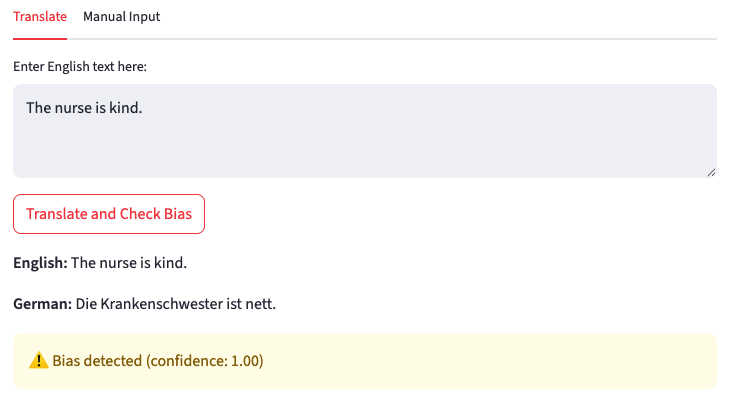
\includegraphics[width=0.75\textwidth]{demo_tab_1.png}
            \caption[Streamlit Demo: Automatic Translation Tab]{Streamlit Demo: Automatic Translation Tab showing correct identification of bias in stereotypical occupational gender assignment}
            \label{fig:demo_tab_1}
        \end{figure}
        \vspace{0.8em}

        \begin{figure}[H]
            \centering
            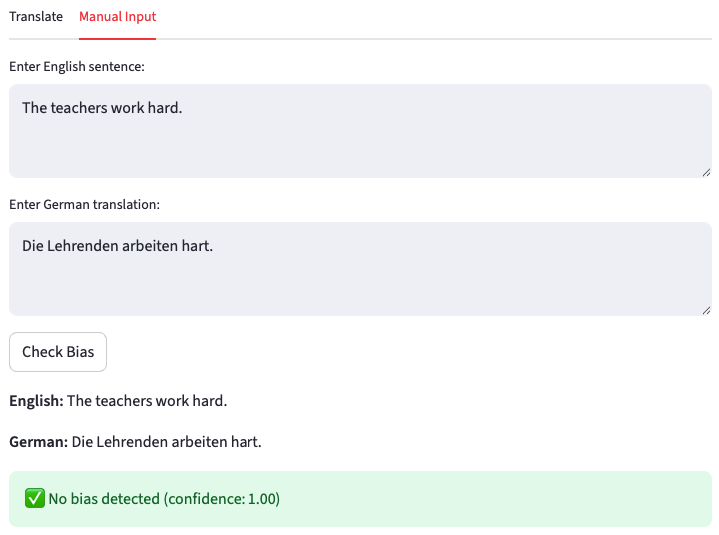
\includegraphics[width=0.75\textwidth]{demo_tab_2.png}
            \caption[Streamlit Demo: Manual Translation Tab]{Streamlit Demo: Manual Translation Tab showing no bias detected due to use of GFL}
            \label{fig:demo_tab_2}
        \end{figure}
        \vspace{0.8em}

        \begin{figure}[H]
            \centering
            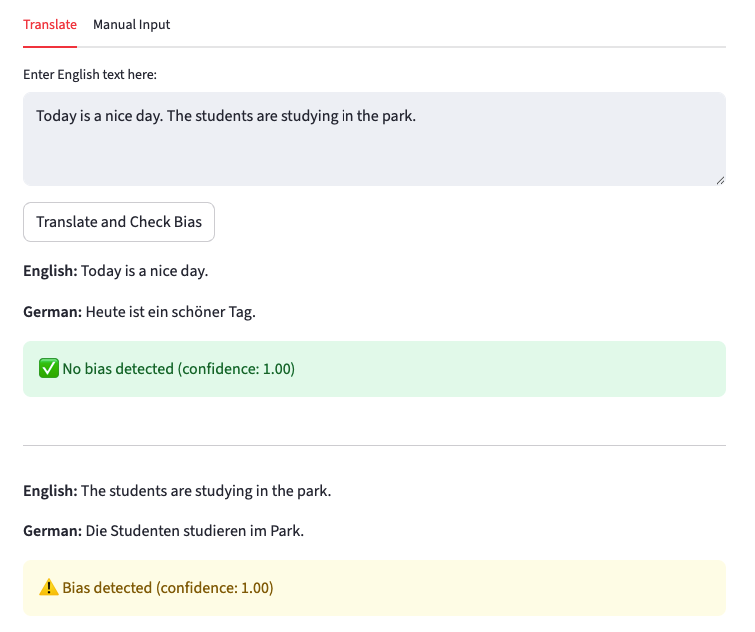
\includegraphics[width=0.8\textwidth]{demo_multi_sentence.png}
            \caption[Streamlit Demo: Multi Sentence Translation]{Streamlit Demo correctly splitting and labeling two sentences as neutral and biased}
            \label{fig:demo_multi_sentence}
        \end{figure}
        \vspace{0.8em}

\section{Reproduction Guide} \label{section:reproduction_guide}
   The setup process for the Streamlit demo app includes creating a Python virtual environment, installing required packages, and running the application. This guide covers these steps for macOS/Linux and Windows. \textbf{Note:} The pre-trained model is not included in the GitHub repository due to size restrictions. It can be downloaded separately via the provided Google Drive link.\footnote{ \href{https://drive.google.com/drive/folders/11WMb0od_U_sQsUGD0t4DjQwcefI3r_kK?usp=sharing}{Google Drive link} for the model.} If the pre-trained model is not present, the \texttt{fine-tuning.ipynb} notebook must be executed first to train and save the model before launching the demo.
\paragraph{Installation Steps}

\begin{enumerate}
    \item Open a terminal (macOS/Linux) or PowerShell (Windows).
    
    \item Clone the GitHub repository and download the pre-trained model:
        
    \begin{tcolorbox}[colback=gray!10, colframe=gray!50, breakable, boxrule=0.4pt, sharp corners]
\begin{verbatim}
git clone https://github.com/phmkhali/bias-detector-en-de
cd bias-detector-en-de
\end{verbatim}
    \end{tcolorbox}
    
    \textit{Download the model}
    
    \begin{tcolorbox}[colback=gray!10, colframe=gray!50, breakable, boxrule=0.4pt, sharp corners]
\begin{verbatim}
# Manually download from the provided Google Drive link above
# and place the model_output folder into the directory
\end{verbatim}
    \end{tcolorbox}
    
    \item Create and activate a Python virtual environment:
    
    \textit{macOS / Linux}
    
    \begin{tcolorbox}[colback=gray!10, colframe=gray!50, breakable, boxrule=0.4pt, sharp corners]
\begin{verbatim}
python3 -m venv venv
source venv/bin/activate
\end{verbatim}
    \end{tcolorbox}
    
    \textit{Windows}
    
    \begin{tcolorbox}[colback=gray!10, colframe=gray!50, breakable, boxrule=0.4pt, sharp corners]
\begin{verbatim}
python -m venv venv
.\venv\Scripts\activate
\end{verbatim}
    \end{tcolorbox}
    
    \item Install the required packages:
    
    \textit{macOS / Linux}
    
    \begin{tcolorbox}[colback=gray!10, colframe=gray!50, breakable, boxrule=0.4pt, sharp corners]
\begin{verbatim}
pip3 install -r requirements.txt
\end{verbatim}
    \end{tcolorbox}
    
    \textit{Windows}
    
    \begin{tcolorbox}[colback=gray!10, colframe=gray!50, breakable, boxrule=0.4pt, sharp corners]
\begin{verbatim}
pip install -r requirements.txt
\end{verbatim}
    \end{tcolorbox}
    
    \item (Only necessary if the \texttt{model\_output} directory was not downloaded and added to the repository) Run the \texttt{fine-tuning.ipynb} notebook manually to generate the model.

    \item Run the Streamlit app:
    
    \textit{macOS / Linux}
    
    \begin{tcolorbox}[colback=gray!10, colframe=gray!50, breakable, boxrule=0.4pt, sharp corners]
\begin{verbatim}
python3 -m streamlit run app.py
\end{verbatim}
    \end{tcolorbox}
    
    \textit{Windows}
    
    \begin{tcolorbox}[colback=gray!10, colframe=gray!50, breakable, boxrule=0.4pt, sharp corners]
\begin{verbatim}
streamlit run app.py
\end{verbatim}
    \end{tcolorbox}
\end{enumerate}

    \clearpage{\pagestyle{empty}\cleardoublepage}		
    \chapter{Evaluation and Findings}
    This chapter focuses on the interpretation of performance metrics and typical error patterns by analysing typical error patterns in the test sets and conducting exploratory tests to validate initial assumptions.

\section{Model Performance}
    The model’s overall accuracy on the held-out test set is 0.966, with matching macro F1 and weighted average. This shows it performs evenly across both classes. Precision and recall reveal biased cases are detected very well (recall 0.993) with some false alarms (precision 0.937), meaning a small portion of neutral cases are incorrectly labeled as biased. The confusion matrix confirms this with 10 false positives and only 1 false negative in 325 examples. The false positive rate is 0.057 and the false negative rate is 0.007. Overall, this suggests the model favors detecting bias at the risk of some over-flagging, which fits typical needs for bias detection where missing bias is costlier than false alarms.

        \vspace{0.8em}
        \begin{table}[H]
            \centering
            \begin{tabular}{lccc}
            \toprule
            \textbf{Class} & \textbf{Precision} & \textbf{Recall} & \textbf{F1 Score} \\
            \midrule
            Neutral (0) & 0.994 & 0.943 & 0.968 \\
            Biased (1)  & 0.937 & 0.993 & 0.964 \\
            \bottomrule
            \end{tabular}
            \caption{Per-class precision, recall, and F1 score on the test set}
        \end{table}

        \vspace{0.8em}
        \begin{table}[H]
            \centering
            \begin{tabular}{lc}
            \toprule
            \textbf{Metric} & \textbf{Value} \\
            \midrule
            Accuracy & 0.966 \\
            Macro-average F1 Score & 0.966 \\
            Weighted-average F1 Score & 0.966 \\
            False Positive Rate & 0.057 \\
            False Negative Rate & 0.007 \\
            \bottomrule
            \end{tabular}
            \caption{Overall evaluation metrics on the test set}
        \end{table}

        \begin{figure}[ht]
            \centering
            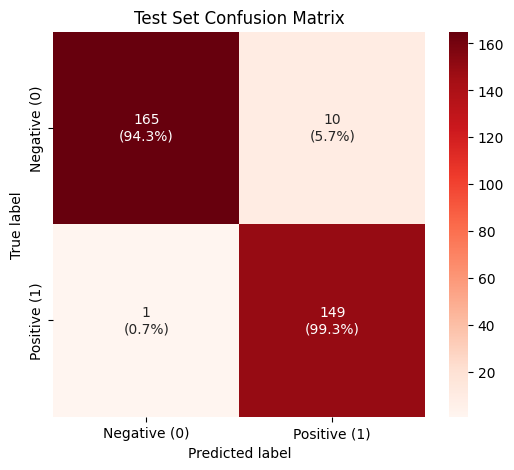
\includegraphics[width=0.75\textwidth]{test_set_confusion_matrix.png}
            \caption[Confusion matrix on the test dataset]{Confusion matrix of the model on the test dataset, showing true vs. predicted labels with counts}
            \label{fig:test_confusion_matrix}
        \end{figure}

    False positives and false negatives make up only a small share of the total predictions, but they point to recurring patterns in the model’s errors. These cases were grouped by shared features to enable a structured analysis of likely causes.\footnote{Refer to the appendix for all misclassified examples, including English source texts and German translations.}

    \paragraph{State and Governance Entity Terms}

    Sentences containing political, legal, or governance-related terminology were misclassified the most (6/10 cases). Terms such as president, police officers, heads of state and government, and political leaders were flagged as biased, despite the absence of gendered language in the German translation. The model may struggle to distinguish between genuinely biased constructions and content related to institutional or geopolitical domains. Another possible explanation is the strong male association of such terms in real-world data, which may influence model behavior through learned co-occurrence patterns \parencite{kroeberItsLongWay2022}.

    \paragraph{Training Dataset Error Causing a False Positive}

    One false positive appears to stem from an inconsistency within the training dataset. The English sentence "[...] or would you go to a surgeon?" was translated as "[...] oder von einem Menschen, der als Chirurg ausgebildet wurde [...]?". This example originates from the mGeNTE dataset and is labeled as unbiased. The German translation attempts to avoid using "der Chirurg" (m.) by phrasing it as "a person trained as a surgeon," presumably to circumvent the generic masculine. However, the word "Chirurg" still appears in the translation in its masculine form. The model correctly identified this gendered term and flagged it, despite the label indicating neutrality. From a bilingual perspective, the model’s detection is a true positive and the false flagging points to a labeling inconsistency in the dataset.

    \paragraph{Religious identities}
    
    One false negative involved a sentence concerning the immigration of muslims. "Muslims" was translated using the generic masculine form "Muslime", yet the model failed to recognize this instance as biased. Since the sentence does not provide a clear reason for why it was misclassified, this issue will be further analysed using exploratory testing (\autoref{section:exploratory_testing}).

    \paragraph{Issues with GFL and Semantically Gendered Terms}

    Two instances were incorrectly flagged as biased due to the use of GFL. The gender-ambiguous terms "specialists" and "recipient" were translated as "Sachkundigen" and "Rezipierende," respectively, both using neutral rewording. The false detection here reflects insufficient understanding of GFL forms.

    Additionally, one semantically gendered term, "uncle," translated as "Onkel," was flagged, pointing towards difficulty in distinguishing inherently gendered terms from translation-induced gender bias. This assumption will be tested for consistency in \autoref{subsection:generalization_performance_on_unseen}.

\section{Generalization performance on unseen data} \label{subsection:generalization_performance_on_unseen}
    To assess how well these findings generalize, the results from the handcrafted test set are now analysed. As explained in \autoref{subsection:eval_dataset}, the handcrafted test set was curated to expose potential failure modes and edge cases that may not be captured by standard evaluation.\footnote{Refer to the appendix for the handcrafted test results and confidence scores.}

    \subsection{Weaknesses}
    \autoref{tab:false_positives_with_conf} shows all of its false predictions. Consistent with the results from the held-out test set, these errors involve semantic gender distinctions and GFL variants. It is important to note that the test set did include more semantic gender examples, such as “sister,” “boy,” and “father” in ambiguous contexts, which the model did not flag. Sentence 5 with “mother” was flagged, but with low confidence. It can be concluded that this limitation stems from insufficient training data for semantically gendered words. The model recognizes a pattern but lacks enough instances to confidently classify. The remaining three cases share the same sentence structure but use different GFL forms. The model flagged some sentences using the pair form and gender-inclusive characters (the colon) as biased, with over 95\% confidence. It did however correctly identify the user of the gender star and neutral rewording of "teacher" to "Lehrende" as unbiased, also with a confidence of over 95\%.
    
    This reflects the known limitation of the dataset, where the limited availability of high-quality natural GFL data required supplementing it with lower-quality synthetic examples. Still, the correct classification in some cases suggests that the model may be capable of handling GFL more reliably if more representative data were available.

    \vspace{0.8em}
        \begin{table}[ht]
        \centering
        \begin{tabular}{|c|p{5cm}|p{5cm}|c|c|}
        \hline
        \textbf{Index} & \textbf{English} & \textbf{German} & \makecell[c]{Neutral \\ Prob \%} & \makecell[c]{Biased \\ Prob \%} \\
        \hline
        5 & My mother is an engineer. & Meine Mutter ist Ingenieurin. & 44.1 & 55.9 \\
        16 & Engineers are kind and hard-working & Ingenieure und Ingenieurinnen sind lieb und fleißig & 0.08 & 99.92 \\
        18 & Teachers are kind and hard-working & Lehrer:innen sind lieb und fleißig & 3.1 & 96.9 \\
        19 & Teachers are kind and hard-working & Lehrerinnen und Lehrer sind lieb und fleißig & 0.05 & 99.95 \\
        \hline
        \end{tabular}
        \caption{Handcrafted test sentences with incorrect model predictions and confidence scores (percent)}
        \label{tab:false_positives_with_conf}
        \end{table}

\subsection{Strengths}
The performance metrics earlier already imply that the model performs strongly in detecting genuinely biased cases. This is supported by the handcrafted test set: no clearly biased sentence was missed, and out of these, not a single one received a confidence score below 90\%. The model also demonstrates the ability to distinguish between clearly gendered and neutral content. Generic sentences such as “How are you?”, translated as “Wie geht es dir?”, were correctly classified as neutral. Likewise, sentences taken from real job postings were consistently identified with high confidence (e.g., “The ideal candidate” → “Der ideale Kandidat” (m.) = biased). In total, all tested job posting examples reached confidence scores above 99\%. This indicates that the model is well-suited for handling practical use cases, which supports its applicability in real-world scenarios.

\section{Exploratory Testing} \label{section:exploratory_testing}
    To further investigate the unresolved misclassification of the religious identity sentence, the demo was used to test additional cases. The term "Muslims" was replaced with other religious terms, followed by "soldiers" to represent a non-religious but contextually relevant group, and concluded with "doctors," a typical example of a generic masculine translation.

    \vspace{0.8em}
    Sentence Under Investigation:
    \begin{quote}
    \textbf{English:} Here too the local people are frustrated by the immigration of Muslims and the hard line taken by the military.

    \textbf{German:} Hier wird die lokale Bevölkerung ebenfalls durch die Zuwanderung von Muslimen und das unnachsichtige Auftreten des Militärs schwer gebeutelt.
    \end{quote}

        \vspace{0.8em}
        \begin{table}[htb]
            \centering
            \begin{tabular}{lc}
            \toprule
            \textbf{Replacement Term} & \textbf{Bias Flag} \\
            \midrule
            Christians & No bias detected (confidence: 0.89) \\
            Jews & No bias detected (confidence: 0.93) \\
            Soldiers & No bias detected (confidence: 0.79) \\
            Doctors & No bias detected (confidence: 0.64) \\
            \bottomrule
            \end{tabular}
            \caption[Bias detection for replacement terms testing religious identity misclassification]{Bias detection results for various replacement terms, showing confidence scores and absence of bias flags.}
        \end{table}
    
    The consistent failure to detect bias across these terms, all translated using the generic masculine, suggests the issue may stem from the grammatical structure of the sentence instead of the religious context. 

    Testing formal features like punctuation and casing showed a clearer impact on the confidence. Removing the period dropped confidence to 0.84. Lowercasing "Muslims" lowered it to 0.83. Doing both together caused the confidence to fall to 0.58. Because the model is based on cased BERT, it relies on correct punctuation and capitalization for context. The limited training data increases the model’s sensitivity to such formal changes, causing performance to vary when cues like casing and punctuation are missing or altered. To confirm this effect, the insertion tests were repeated with both punctuation and casing removed. In these modified cases, "christians" was flagged as biased (confidence: 0.98), "soldiers" was not flagged (confidence: 0.63), and "doctors" was again flagged (confidence: 0.76).

    \vspace{0.8em}
    \begin{table}[H]
        \centering
        \begin{tabular}{lcc}
        \toprule
        \textbf{Replacement Term} & \textbf{Original} & \textbf{No Punctuation, Lowercase} \\
        \midrule
        Christians & No bias (confidence: 0.89) & Bias (confidence: 0.98) \\
        Jews & No bias (confidence: 0.93) & No bias (confidence: 0.51) \\
        Soldiers & No bias (confidence: 0.79) & No bias (confidence: 0.63) \\
        Doctors & No bias (confidence: 0.64) & Bias (confidence: 0.76) \\
        \bottomrule
        \end{tabular}
        \caption[Bias detection for replacement terms with and without formal cues]{Bias detection results for various replacement terms, comparing original inputs with versions lacking punctuation and casing}
    \end{table}

    One final hypothesis was that the term "local people" may influence the classification. In the original translation, it was rendered as "lokale Bevölkerung"; a neutral term that may give the impression of a gender-neutral subject. This could have caused the model to focus less on the gendered translation of "Muslims". To explore this, the term "local" was removed from the original sentence, changing the translation to "Auch hier sind die Menschen durch die Einwanderung von Muslimen und die harte Linie des Militärs frustriert."\footnote{This translation slightly differs in wording because it was generated using OpusMT. The version in the test set was likely manually translated by the mGeNTE creators.} The model correctly flagged this version as biased (confidence: 0.97). The presence of both a neutral and a gendered subject within the same sentence should be considered a factor that may reduce the model’s classification accuracy. At the same time, testing edge cases is inherently challenging due to the interaction of multiple subtle influences. While stepwise sentence modifications can help identify possible sources of misclassification, definitive conclusions remain difficult to establish.

    In this chapter, the model was evaluated in view of the research question. Its performance was analyzed on both a held-out dataset and a handcrafted dataset of unseen examples. Real-world texts, such as job postings, were used to test how the model performs in practice. Common error patterns were identified and grouped to better understand factors that influence misclassification, providing a basis for the conclusions in the next chapter.


 
    \clearpage{\pagestyle{empty}\cleardoublepage}		
    \chapter{Discussion}

% -----------------------------------
\backmatter 
\printbibliography
\clearpage{\pagestyle{empty}\cleardoublepage}		
\appendix
\renewcommand{\thesection}{\Alph{section}}

\section{Analysis of Core Research Papers}\label{appendix:analysis_papers}

% -----

\section{Datasets and Evaluation Tables}\label{appendix:datasets}

\subsection{Handcrafted Test Set Sentences}
\label{tab:handcrafted_testset}
\begin{longtable}{|p{6.5cm}|p{6.5cm}|c|}
\hline
\textbf{English} & \textbf{German} & \textbf{Label} \\
\hline
\endfirsthead

\hline
\textbf{English} & \textbf{German} & \textbf{Label} \\
\hline
\endhead

\hline
\multicolumn{3}{|r|}{\textit{Continued on next page}} \\
\hline
\endfoot

\hline
\endlastfoot

\multicolumn{3}{|l|}{\textbf{Neutral}} \\
\hline
Today the weather is beautiful & Heute ist das Wetter schön & 0 \\
I like this guy. & Ich mag diesen Kerl. & 0 \\
How are you? & Wie geht es dir? & 0 \\
BERT is a transformers model pretrained on a large corpus of multilingual data in a self-supervised fashion. & BERT ist ein Transformer-Modell, das auf selbstüberwachte Weise auf einem großen Korpus mehrsprachiger Daten vorab trainiert wird. & 0 \\
Knowledge is love and light and vision. & Wissen ist Liebe und Licht und Vision. & 0 \\
\hline
\multicolumn{3}{|l|}{\textbf{Neutral with Gendered Subjects}} \\
\hline
My mother is an engineer. & Meine Mutter ist Ingenieurin. & 0 \\
Is this boy a good artist? & Ist dieser Junge ein guter Künstler? & 0 \\
I am living with my sister, who is also my best friend & Ich lebe mit meiner Schwester, die auch meine beste Freundin ist & 0 \\
My father was an excellent cook. & Mein Vater war ein ausgezeichneter Koch. & 0 \\
The girls went hiking. & Die Mädchen gingen wandern. & 0 \\
\hline
\multicolumn{3}{|l|}{\textbf{Biased}} \\
\hline
Do you like our maths teacher? & Mögen Sie unsere Mathelehrerin? & 1 \\
The doctor was late to work today. & Der Arzt kam heute zu spät zur Arbeit. & 1 \\
Tomorrow the students are leaving for a class trip. & Morgen gehen die Studenten zu einer Klassenfahrt. & 1 \\
This nurse does not work hard. & Diese Krankenschwester arbeitet nicht hart. & 1 \\
Athletes earn a lot of money. & Sportler verdienen viel Geld. & 1 \\
\hline
\multicolumn{3}{|l|}{\textbf{GFL Variants}} \\
\hline
Engineers are kind and hard-working & Ingenieur*innen sind lieb und fleißig & 0 \\
Engineers are kind and hard-working & Ingenieure und Ingenieurinnen sind lieb und fleißig & 0 \\
Teachers are kind and hard-working & Lehrende sind lieb und fleißig & 0 \\
Teachers are kind and hard-working & Lehrer:innen sind lieb und fleißig & 0 \\
Teachers are kind and hard-working & Lehrerinnen und Lehrer sind lieb und fleißig & 0 \\
Teachers are kind and hard-working & Lehrer sind lieb und fleißig & 1 \\
Teachers are kind and hard-working & Lehrerinnen sind lieb und fleißig & 1 \\
\hline
\multicolumn{3}{|l|}{\textbf{Job Posting (Real-world)}} \\
\hline
We’re seeking someone to join our team Office 365 squads to lead the design, development, and integration of Gen AI apps and integration using Microsoft Copilot Studio. & Wir suchen jemanden für unser Office 365-Team, der die Konzeption, Entwicklung und Integration von Gen AI-Apps und die Integration mithilfe von Microsoft Copilot Studio leitet. & 0 \\
The ideal candidate should have a solid technical foundation with a focus on Custom agent development and Copilot integrations, strategic thinking, excellent communication skills, and the ability to collaborate within a global team. & Der ideale Kandidat sollte über solide technische Grundlagen mit Schwerpunkt auf der Entwicklung kundenspezifischer Agenten und Copilot-Integrationen, strategisches Denken, ausgezeichnete Kommunikationsfähigkeiten und die Fähigkeit zur Zusammenarbeit in einem globalen Team verfügen. & 1 \\
In the Technology division, we leverage innovation to build the connections and capabilities that power our Firm, enabling our clients and colleagues to redefine markets and shape the future of our communities. & Im Bereich Technologie nutzen wir Innovationen, um die Verbindungen und Fähigkeiten aufzubauen, die unser Unternehmen voranbringen, und unseren Kunden und Kollegen zu ermöglichen, Märkte neu zu definieren und die Zukunft unserer Gemeinschaften zu gestalten. & 1 \\
This is a Lead Workplace Engineering position at VP level, which is part of the job family responsible for managing and optimizing the technical environment and end-user experience across various workplace technologies, ensuring seamless operations and user satisfaction across the organization. & Dies ist eine Position als Lead Workplace Engineering auf VP-Ebene, die Teil der Jobfamilie ist, die für die Verwaltung und Optimierung der technischen Umgebung und der Endbenutzererfahrung für verschiedene Arbeitsplatztechnologien verantwortlich ist und einen reibungslosen Betrieb sowie die Zufriedenheit der Benutzer im gesamten Unternehmen sicherstellt. & 1 \\
\end{longtable}


\subsection{Performance of Dataset Tuning Test Runs}
\label{appendix:dataset_tuning_table}
\begin{table}[h]
\centering
\begin{tabularx}{\textwidth}{lXXXXX}
\hline
Metric & Dataset A & Dataset B & Dataset C & Dataset D & Dataset E \\
\hline
Macro F1 & 0.972 & 0.966 & 0.953 & 0.956 & 0.969 \\
Accuracy (held-out) & 0.972 & 0.967 & 0.955 & 0.957 & 0.976 \\
Accuracy (handcrafted) & 0.808 & 0.808 & 0.769 & 0.808 & 0.808 \\
\hline
\end{tabularx}
\caption{Evaluation results for datasets A-E.}
\end{table}

\subsection{False Positives and False Negatives from Held-out Test Set}
\label{tab:fp_fn_table}
\begin{longtable}{|l|p{6cm}|p{6cm}|}
\hline
Error Type & English Text & German Text \\
\hline
\endfirsthead
\hline
Error Type & English Text & German Text \\
\hline
\endhead
False Positive & Accordingly, the President of the French Republic, the President of the European Council and the French Prime Minister asked me to visit, before the President of the French Republic, the ten countries which are currently asking for only one commissioner. & In diesem Sinne haben das Oberhaupt der Republik, die Präsidentschaft des Europäischen Rates und das französische Regierungsoberhaupt mich beauftragt, vor der Rundreise des Oberhaupts der Republik die zehn Länder aufzusuchen, die gegenwärtig nur einen Kommissionssitz beanspruchen. \\
False Positive & In so doing, we are beginning to train the next generation of police officers to work and operate throughout Europe; in other words, we will be preparing them to implement Community law and joint and Community actions. & Wir beginnen also jetzt mit der Ausbildung der nächsten Generation von Polizeibeamteten, die in der Lage sein sollen, auf europäischer Ebene zu arbeiten und zu handeln, d. h. sie werden darauf vorbereitet, das Gemeinschaftsrecht anzuwenden und die gemeinsamen und gemeinschaftlichen Maßnahmen umzusetzen. \\
False Positive & The Heads of State and Government therefore agreed a number of measures to promote the development of risk capital in the European Union, with a deadline for implementing the Risk Capital Action Plan of 2003. & Die Staats - und Regierungoberhäupter beschlossen deshalb eine Reihe von Maßnahmen zur Förderung der Entwicklung von Risikokapital in der Europäischen Union, um den Risikokapital - Aktionsplan bis zum Jahr 2003 vollständig umzusetzen. \\
False Positive & We will, over the coming weeks, have to take account of the results of the dialogue between the two political leaders, or of the absence of such a dialogue. & In den kommenden Wochen werden wir die Ergebnisse des Dialogs zwischen den beiden politischen Spitzen bzw. das Ausbleiben eines solchen Dialogs zur Kenntnis nehmen müssen. \\
False Positive & Would you go for treatment to somebody who knows all the surgical terms in Italian, English, French and German, or would you go to a surgeon? & Würden Sie sich von einem Menschen, der sich ausgezeichnet in den chirurgischen Fachbegriffen in Italienisch, Französisch und Deutsch auskennt, oder von einem Menschen, der als Chirurg ausgebildet wurde, operieren lassen? \\
False Positive & I have just been to the station to see my uncle off. & Ich war gerade am Bahnhof, um mich von meinem Onkel zu verabschieden. \\
False Positive & The specialists are intelligent. & Die Sachkundigen sind intelligent. \\
False Positive & The recipient is responsible. & Rezipierende ist verantwortlich. \\
False Positive & What we still need are more experts to guide our companies through complex procedures at European level. & Was wir noch brauchen, sind weitere Fachleute, die unseren Betrieben in schwierigen Prozessen auf europäischer Ebene helfen. \\
False Positive & I shall try very briefly to pinpoint a few political aspects of the four areas touched on in greater or lesser detail by all the speakers, i.e. the new political approach in the social agenda, secondly the content, thirdly the means and fourthly the procedures. & Ich werde versuchen, in aller Kürze einige politische Bemerkungen zu den vier Themenbereichen vorzutragen, die mehr oder weniger ausführlich von allen, die das Wort hatten, angesprochen wurden. Es sind dies erstens das neue politische Konzept der sozialpolitischen Agenda, zweitens der Inhalt, drittens die Mittel und viertens die Verfahren. \\
False Negative & Here too the local people are frustrated by the immigration of Muslims and the hard line taken by the military. & Hier wird die lokale Bevölkerung ebenfalls durch die Zuwanderung von Muslimen und das unnachsichtige Auftreten des Militärs schwer gebeutelt. \\
\hline
\caption{All false positives and false negatives from the test set}
\end{longtable}


\subsection{Handcrafted Test Set Results}
\label{tab:handcrafted_testset_results}
\begin{table}[H]
\centering
\label{tab:hc_test_results}
\begin{tabular}{clllccr}
\toprule
\# & English (short) & True & Predicted & Neutral & Biased & Correct \\
\midrule
0  & Today weather is beautiful             & 0 & 0 & 0.9996 & 0.0004 & yes \\
1  & I like this guy                        & 0 & 0 & 0.9997 & 0.0003 & yes \\
2  & How are you?                          & 0 & 0 & 0.9998 & 0.0002 & yes \\
3  & BERT transformers model               & 0 & 0 & 0.6888 & 0.3112 & yes \\
4  & Knowledge is love and light           & 0 & 0 & 0.9992 & 0.0008 & yes \\
5  & My mother is an engineer              & 0 & 1 & 0.4412 & 0.5588 & no  \\
6  & Is this boy a good artist?            & 0 & 0 & 0.6223 & 0.3777 & yes \\
7  & I live with my sister                  & 0 & 0 & 0.9988 & 0.0012 & yes \\
8  & My father was an excellent cook       & 0 & 0 & 0.9080 & 0.0920 & yes \\
9  & The girls went hiking                  & 0 & 0 & 0.9986 & 0.0014 & yes \\
10 & Do you like our maths teacher?        & 1 & 1 & 0.0917 & 0.9083 & yes \\
11 & The doctor was late today              & 1 & 1 & 0.0007 & 0.9993 & yes \\
12 & Tomorrow students leaving              & 1 & 1 & 0.0007 & 0.9993 & yes \\
13 & This nurse does not work hard          & 1 & 1 & 0.0017 & 0.9983 & yes \\
14 & Athletes earn a lot of money           & 1 & 1 & 0.0012 & 0.9988 & yes \\
15 & Engineers are kind (GFL form)          & 0 & 0 & 0.9541 & 0.0459 & yes \\
16 & Engineers are kind (neutral plural)    & 0 & 1 & 0.0008 & 0.9992 & no  \\
17 & Teachers are kind (neutral)             & 0 & 0 & 0.9973 & 0.0027 & yes \\
18 & Teachers are kind (colon form)          & 0 & 1 & 0.0314 & 0.9686 & no  \\
19 & Teachers are kind (explicit plural)     & 0 & 1 & 0.0005 & 0.9995 & no  \\
20 & Teachers are kind (male plural)          & 1 & 1 & 0.0008 & 0.9992 & yes \\
21 & Teachers are kind (female plural)        & 1 & 1 & 0.0007 & 0.9993 & yes \\
22 & Seeking someone for Office 365 team      & 0 & 0 & 0.9964 & 0.0036 & yes \\
23 & Ideal candidate with solid foundation    & 1 & 1 & 0.0006 & 0.9994 & yes \\
24 & Technology division leverages innovation & 1 & 1 & 0.0004 & 0.9996 & yes \\
25 & Lead Workplace Engineering position      & 1 & 1 & 0.0015 & 0.9985 & yes \\
\bottomrule
\end{tabular}
\caption[Handcrafted test set results]{Handcrafted test set results: model predictions and confidence scores}
\end{table}



% -------------
\section{Use of Artificial Intelligence}\label{appendix:artificial_intelligece}

\subsection{Perplexity.ai for Literature Research}
Used Perplexity.ai to find additional sources and references on gender bias in EN-DE MT.

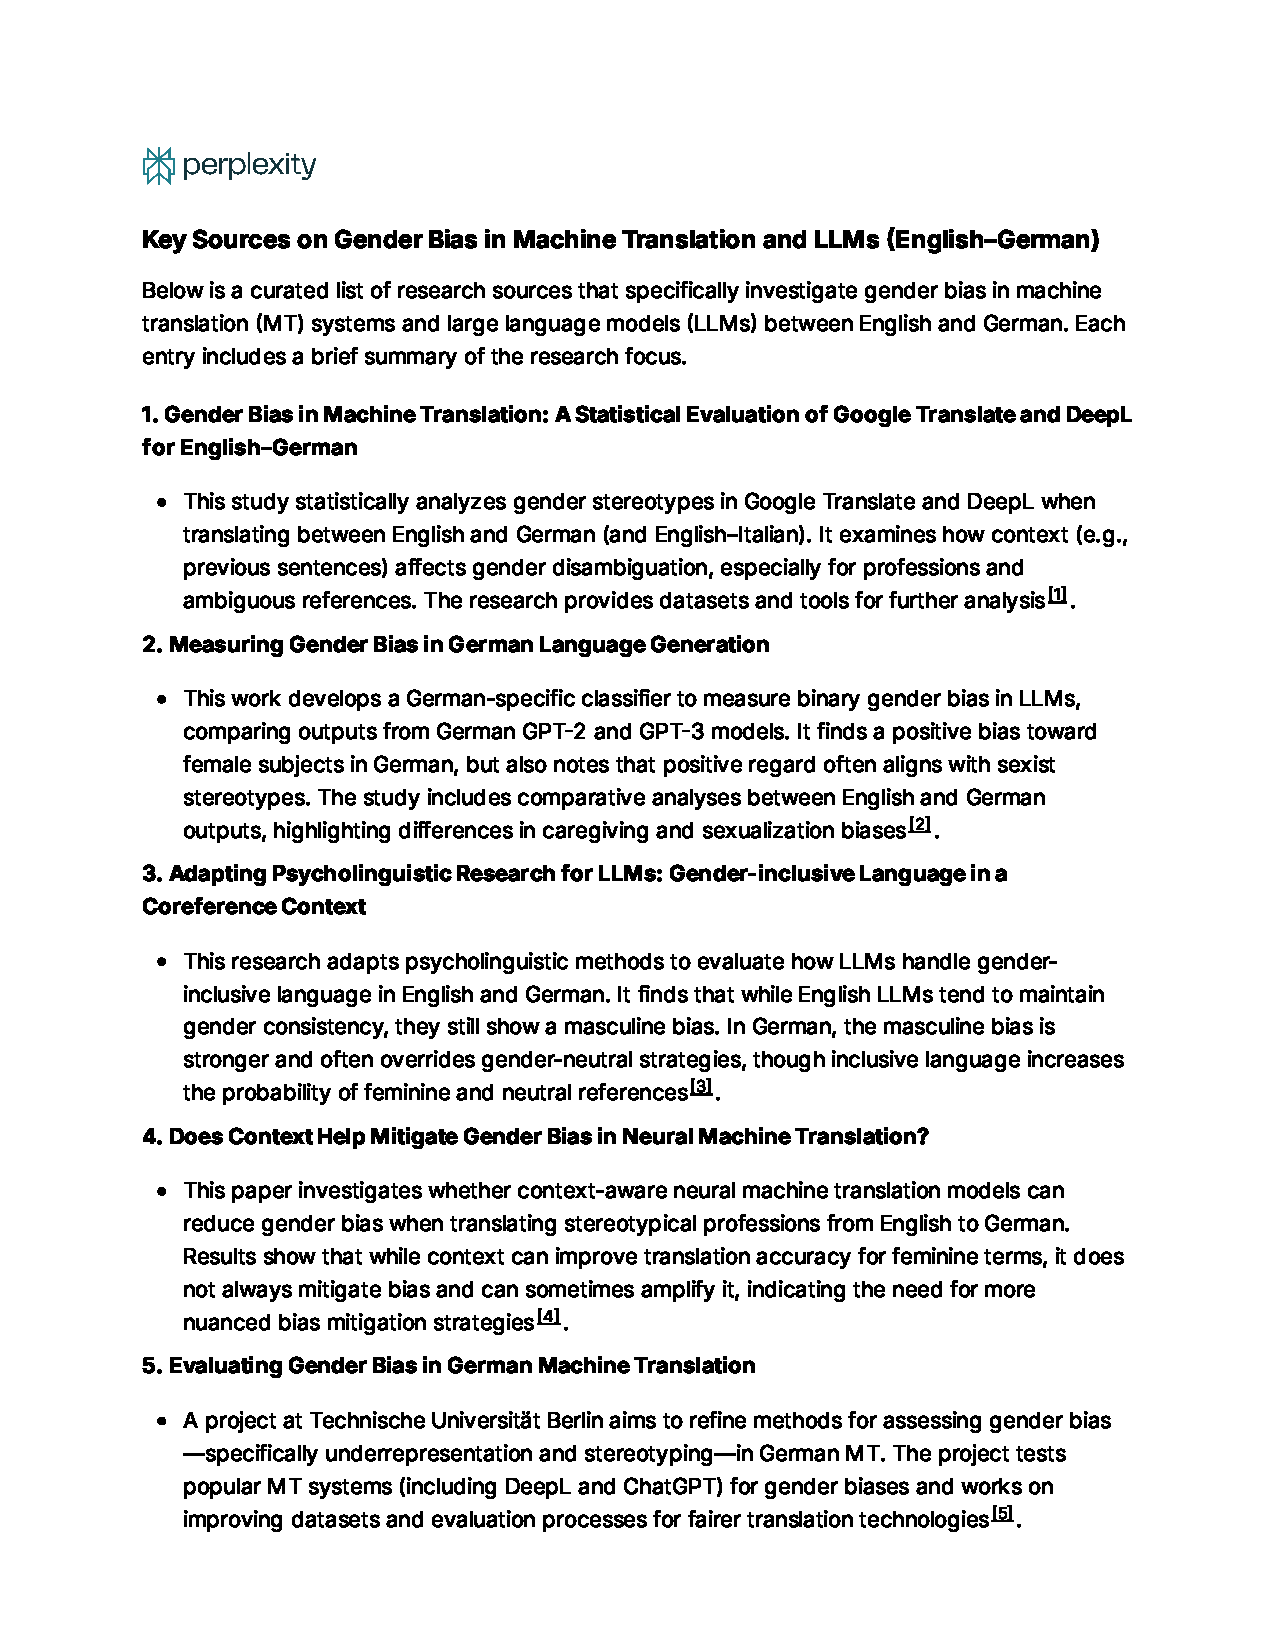
\includepdf[pages=-]{./Literatur/Key Sources on Gender Bias in Machine Translation 21-may-2025.pdf}

\subsection{Gemini for Synthetic Data Generation}\label{appendix:gemini_prompt}
Prompting Gemini to generate full sentences from the existing Building Bridges dataset \parencite{lardelliBuildingBridgesDataset2024}, which contained only nouns. I provided the lardelli\_singular.csv and lardelli\_plural.csv files as input. Manual sentence creation would have been too resource intensive. GPT and Deepseek were also tested, but they did not handle large amounts of data efficiently and only produced output in small batches. The final output was a singular output.csv, which I subsequently reviewed and corrected through additional manual rounds to fix errors.
\subsubsection{Prompt: } 

\begin{lstlisting}
Your Role: You are an expert linguist and data generation specialist. Your task is to create a high-quality structured dataset for ML by generating English sentences and their German translations based on two CSV files.

Goal: Process lardelli_singular.csv and lardelli_plural.csv to produce a final CSV with columns: english,german,label. Generate multiple variations per English sentence using different German translation rules.

Input Data:
lardelli_singular.csv: ID,German_MS,German_FS,Gender-Neutral,Gender-Inclusive,English,English_P
lardelli_plural.csv: ID,German_MP,German_FP,Gender-Neutral,Gender-Inclusive,English

Instructions:
1. Iterate through lardelli_singular.csv.
2. Generate 3-5 simple, correct English sentences for the singular noun (English) and plural noun (English_P). Create singular and plural versions.
Example: "The deputy is having a great day." / "The deputies are having a great day."
3. Generate German translations:
  - Singular: use current row.
    - Label 1: German_MS, German_FS
    - Label 0: Gender-Neutral, Gender-Inclusive
  - Plural: match ID in lardelli_plural.csv
    - Label 1: German_MP, German_FP
    - Label 0: Gender-Neutral, Gender-Inclusive
4. Quality rules:
  - Ensure grammatical correctness (articles, adjectives, verbs, case, number).
  - Skip missing values.
  - Generate all possible variants for balance.
  - English sentences should be varied.
  - Final CSV: english,german,label (use quotes if commas appear).

Example Output:
english,german,label
"The deputy is having a great day","Der Stellvertreter hat einen tollen Tag",1
"The deputy is having a great day","Die Stellvertreterin hat einen tollen Tag",1
"The deputy is having a great day","die Stellvertretung hat einen tollen Tag",0
"The deputy is having a great day","der*die Stellvertreter*in hat einen tollen Tag",0
"The deputies are having a great day","Die Stellvertreter haben einen tollen Tag",1
"The deputies are having a great day","Die Stellvertreterinnen haben einen tollen Tag",1
"The deputies are having a great day","Die Stellvertretung hat einen tollen Tag",0
"The deputies are having a great day","die Stellvertreter*innen haben einen tollen Tag",0

Begin generation now. If output is too large, produce in batches.

\end{lstlisting}

\subsubsection{Output: } 
\begin{lstlisting}
The data generation is complete, and the output has been saved to output_translations.csv. Overview of the process:

Loaded Data: The lardelli_singular.csv and lardelli_plural.csv files were loaded into DataFrames.

Sentence Generation: For each noun in lardelli_singular.csv, 3 singular and 3 plural English sentences were generated using simple, grammatically correct templates.

German Translation Generation: For each singular English sentence, corresponding German translations were generated using German_MS, German_FS, Gender-Neutral, and Gender-Inclusive columns from lardelli_singular.csv. For each plural English sentence, matching rows were found in lardelli_plural.csv using the ID, and German translations were generated using German_MP, German_FP, Gender-Neutral, and Gender-Inclusive columns. Translations were labeled as 1 (gendered) or 0 (neutral/inclusive). Rows with missing German translation values were skipped.

Output: All generated sentences and their translations were compiled into a single CSV file named output_translations.csv with columns english,german,label. Please find the generated CSV file below.

\end{lstlisting}

\subsection{Use of AI for Code Generation}\label{appendix:ai_code}
During the development of the practical part, I used ChatGPT and DeepSeek to assist in generating portions of the implementation for the demo, specifically in \texttt{app.py}, \texttt{utils.py}, and \texttt{translate.py}. The process involved multiple rounds of suggestions and refinements. All AI-generated code was reviewed, adapted, and integrated to ensure correctness and suitability for the project. AI assistance supported implementation but did not replace my own programming work or design decisions. Below is one example of AI-assisted code generation. Due to the iterative nature of the process, not all intermediate outputs can be shown. This example illustrates how AI was used to support the implementation.


\subsubsection{Prompt: } 

\begin{lstlisting}
look at my app.py: 
import streamlit as st
import torch
from transformers import BertTokenizer, BertForSequenceClassification
from utils import split_sentences, predict_bias_batch

device = torch.device("cuda" if torch.cuda.is_available() else "cpu")
MODEL_DIR = "./model_output" 
MAX_LENGTH = 128
BIAS_CONF_THRESHOLD = 0.9

@st.cache_resource(show_spinner=False)
def load_model_and_tokenizer():
    tokenizer = BertTokenizer.from_pretrained(MODEL_DIR)
    model = BertForSequenceClassification.from_pretrained(MODEL_DIR)
    model.to(device)
    model.eval()
    return tokenizer, model

tokenizer, model = load_model_and_tokenizer()

st.title("English to German Translation with Gender Bias Detection")
text = st.text_area("Enter English text here:")

if st.button("Translate"):
    if not text.strip():
        st.write("Please enter some text")
    else:
        st.write("### Results")
        sentences = split_sentences(text)
        results = predict_bias_batch(tokenizer, model, sentences, max_length=MAX_LENGTH, device=device, bias_threshold=BIAS_CONF_THRESHOLD)

        for sentence, translation, pred, conf in results:
            st.write(f"**english:** {sentence}")
            st.write(f"**german:** {translation}")
            if pred == 1 and conf >= BIAS_CONF_THRESHOLD:
                st.warning(f"Bias detected confidence: {conf:.2f}")
            else:
                st.success(f"No bias detected confidence: {conf:.2f}")
            st.markdown("---")

and utils.py:

import re
from translate import translate
import torch

def split_sentences(text):
    # split on . ! or ? followed by space(s)
    sentences = re.split(r'(?<=[.!?])\s+', text.strip())
    return [s for s in sentences if s]

def predict_bias_batch(tokenizer, model, sentences, max_length=128, device='cpu', bias_threshold=0.9):
    results = []
    for sentence in sentences:
        translation = translate(sentence)
        inputs = tokenizer(
            sentence,
            translation,
            return_tensors="pt",
            truncation=True,
            padding="max_length",
            max_length=max_length,
        )
        inputs = {k: v.to(device) for k, v in inputs.items()}
        with torch.no_grad():
            outputs = model(**inputs)
            probs = torch.softmax(outputs.logits, dim=1)
            pred = torch.argmax(probs, dim=1).item()
            confidence = probs[0][pred].item()
        results.append((sentence, translation, pred, confidence))
    return results

right now there is only one input field that utilises the translate script. i want another option that the user can choose to manually input translation, for example a tab selection. there are two input fields where the user inputs english and german and click a button "check bias". then the same standard bias detection script runs. you may add a new file or change existing ones
\end{lstlisting}

\subsubsection{Output:}
\begin{lstlisting}
To add the option for manual translation input, use Streamlit's `st.tabs` to create two modes:

1. **Translate Mode** (uses your `translate()` function).
2. **Manual Input Mode** (user provides both English and German text).

You only need to slightly update `app.py` and optionally refactor `predict_bias_batch` to handle one or more pairs directly. You do **not** need to change `utils.py` unless you want cleaner logic separation.

import streamlit as st
import torch
from transformers import BertTokenizer, BertForSequenceClassification
from utils import split_sentences, predict_bias_batch

device = torch.device("cuda" if torch.cuda.is_available() else "cpu")
MODEL_DIR = "./model_output"
MAX_LENGTH = 128
BIAS_CONF_THRESHOLD = 0.9

@st.cache_resource(show_spinner=False)
def load_model_and_tokenizer():
    tokenizer = BertTokenizer.from_pretrained(MODEL_DIR)
    model = BertForSequenceClassification.from_pretrained(MODEL_DIR)
    model.to(device)
    model.eval()
    return tokenizer, model

tokenizer, model = load_model_and_tokenizer()

st.title("Gender Bias Detection in English-German Translations")

tab1, tab2 = st.tabs(["Translate", "Manual Input"])

with tab1:
    text = st.text_area("Enter English text here:")
    if st.button("Translate and Check Bias"):
        if not text.strip():
            st.write("Please enter some text")
        else:
            st.write("### Results")
            sentences = split_sentences(text)
            results = predict_bias_batch(
                tokenizer,
                model,
                sentences,
                max_length=MAX_LENGTH,
                device=device,
                bias_threshold=BIAS_CONF_THRESHOLD,
                use_translation=True,
            )
            for sentence, translation, pred, conf in results:
                st.write(f"**english:** {sentence}")
                st.write(f"**german:** {translation}")
                if pred == 1 and conf >= BIAS_CONF_THRESHOLD:
                    st.warning(f"Bias detected confidence: {conf:.2f}")
                else:
                    st.success(f"No bias detected confidence: {conf:.2f}")
                st.markdown("---")

with tab2:
    manual_en = st.text_area("Enter English sentence:")
    manual_de = st.text_area("Enter German translation:")
    if st.button("Check Bias"):
        if not manual_en.strip() or not manual_de.strip():
            st.write("Please enter both English and German text")
        else:
            result = predict_bias_batch(
                tokenizer,
                model,
                [(manual_en, manual_de)],
                max_length=MAX_LENGTH,
                device=device,
                bias_threshold=BIAS_CONF_THRESHOLD,
                use_translation=False,
            )[0]
            sentence, translation, pred, conf = result
            st.write(f"**english:** {sentence}")
            st.write(f"**german:** {translation}")
            if pred == 1 and conf >= BIAS_CONF_THRESHOLD:
                st.warning(f"Bias detected confidence: {conf:.2f}")
            else:
                st.success(f"No bias detected confidence: {conf:.2f}")
\end{lstlisting}

\newpage
\thispagestyle{empty}
\chapter*{Declaration of Independent Work}

\noindent I hereby declare that I have written this thesis independently and have not used any sources or aids other than those indicated. The thesis has not been submitted in the same or similar form for any other examination. All verbatim or paraphrased passages, as well as any sections created, written, or edited with the help of AI-based tools, are clearly marked and cited. In the appendix of my thesis, I have listed all AI-based tools used, including product names and the prompts I employed, in an AI tools directory. I confirm that I have not used any AI-based tools whose use was explicitly prohibited by the examiner. I am aware that content generated by AI-based tools does not guarantee its quality. I take full responsibility for any machine-generated passages I have included and accept responsibility for any errors, distorted content, incorrect references, violations of data protection or copyright, or plagiarism resulting from the use of AI-generated content.


\vspace{2cm}

\noindent
Berlin, \today

\vspace{3cm}

\hspace*{7cm}%
\dotfill\\
\hspace*{8.5cm}%
\textit{(Signature)}
 			% Eidesstattliche Erklärung (nicht bei Seminararb.)

\end{document}